%%%%%%%%%%%%%%%%%%%%%%%%%%%%%%%%%%%%%%%%%%%%%%%%%%%%%%%%%%%%%%%%%%%%%%%%%%%%%%%%
%2345678901234567890123456789012345678901234567890123456789012345678901234567890
%        1         2         3         4         5         6         7         8

\documentclass[letterpaper, 10 pt, conference]{ieeeconf}  % Comment this line out if you need a4paper

%\documentclass[a4paper, 10pt, conference]{ieeeconf}      % Use this line for a4 paper

\IEEEoverridecommandlockouts                              % This command is only needed if 
% you want to use the \thanks command

\overrideIEEEmargins                                      % Needed to meet printer requirements.

% See the \addtolength command later in the file to balance the column lengths
% on the last page of the document

% The following packages can be found on http:\\www.ctan.org
\usepackage{graphics} % for pdf, bitmapped graphics files
\usepackage{epsfig} % for postscript graphics files
%\usepackage{mathptmx} % assumes new font selection scheme installed
%\usepackage{times} % assumes new font selection scheme installed
\usepackage{amsmath} % assumes amsmath package installed
\usepackage{amssymb}  % assumes amsmath package installed
\usepackage{bm}
\usepackage[caption=false]{subfig}
\usepackage{algpseudocode}
\usepackage[table]{xcolor}

\newsavebox{\ieeealgbox}
\newenvironment{boxedalgorithmic}
  {\begin{lrbox}{\ieeealgbox}
   \begin{minipage}{\dimexpr\columnwidth-2\fboxsep-2\fboxrule}
   \begin{algorithmic}}
  {\end{algorithmic}
   \end{minipage}
   \end{lrbox}\noindent\fbox{\usebox{\ieeealgbox}}}



\newcommand{\x}{\mbox{$\mathbf x$}}
\newcommand{\btheta}{\mbox{$\bm \theta$}}
\newcommand{\fsym}{\mbox{$\mathbf z$}}
\newcommand{\fsd}{\mbox{$\mathbf z_{\text{sd}}$}}
\newcommand{\fssd}{\mbox{$\mathbf z_{\text{ssd}}$}}
\newcommand{\fcon}{\mbox{$\mathbf z_{\text{con}}$}}
\newcommand{\fsht}{\mbox{$\mathbf z_{\text{sht}}$}}
\newcommand{\fconv}{\mbox{$\mathbf z_{\text{conv}}$}}

\title{\LARGE \bf
  Predicting Initialization Effectiveness for Trajectory Optimization
}


\author{Jia Pan \and Zhuo Chen \and Pieter Abbeel \thanks{Authors are with the Department of Electrical Engineering and Computer Science, University of California at Berkeley, CA, USA.}}


\begin{document}



\maketitle
\thispagestyle{empty}
\pagestyle{empty}


%%%%%%%%%%%%%%%%%%%%%%%%%%%%%%%%%%%%%%%%%%%%%%%%%%%%%%%%%%%%%%%%%%%%%%%%%%%%%%%%
\begin{abstract}
Trajectory optimization is a method for solving motion planning problems by formulating them as non-convex constrained optimization problems. The optimization process, however, can get stuck in local optima that are in collision. As a consequence, these methods typically require multiple initializations.  This poses the problem of deciding which initializations to use when given a limited computational budget. In this paper we propose a machine learning approach to predict whether a collision-free solution will be found from a given initialization. We present a set of trajectory features that encode the obstacle distribution locally around a robot. These features are designed for generalization across different tasks.  Our experiments on various planning benchmarks demonstrate the performance of our approach.
\end{abstract}


\section{Introduction}
Trajectory optimization algorithms are becoming attractive options for robotic motion planning, especially for problems with many degrees of freedom (DOF). Given an initial trajectory that may contain collisions and violate constraints, trajectory optimization methods can often quickly converge to a high-quality, locally-optimal solution. These methods are readily able to incorporate dynamics, smoothness and obstacle avoidance.

Despite their success in various applications, trajectory optimization techniques suffer from a critical limitation: their performance heavily depends on the choice of initial trajectories. For instance, certain initializations passing through obstacles in unfavorable ways may get stuck in infeasible solutions and cannot resolve all collisions in the final outcome, as illustrated in Figure~\ref{fig:failexamples}. As we discuss later, trajectories that pass through the medial axis of an obstacle are prone to getting stuck in a local optimum.

\begin{figure}[!h]
\centering
\subfloat[initial path]{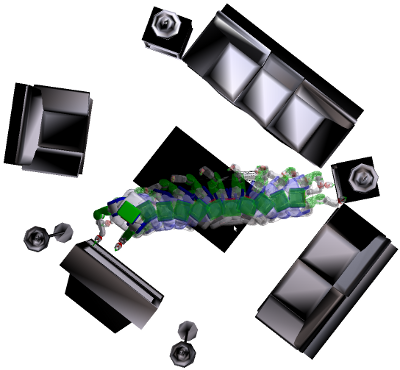
\includegraphics[width=0.38\linewidth]{figure/1.png}} \qquad
\subfloat[result path]{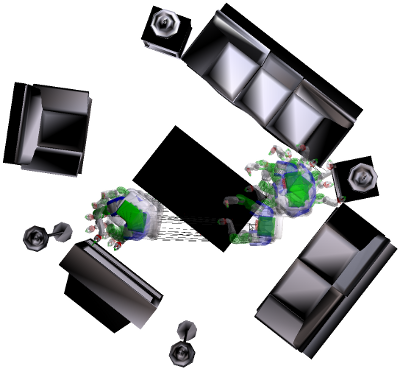
\includegraphics[width=0.38\linewidth]{figure/2.png}} \\
\subfloat[initial path]{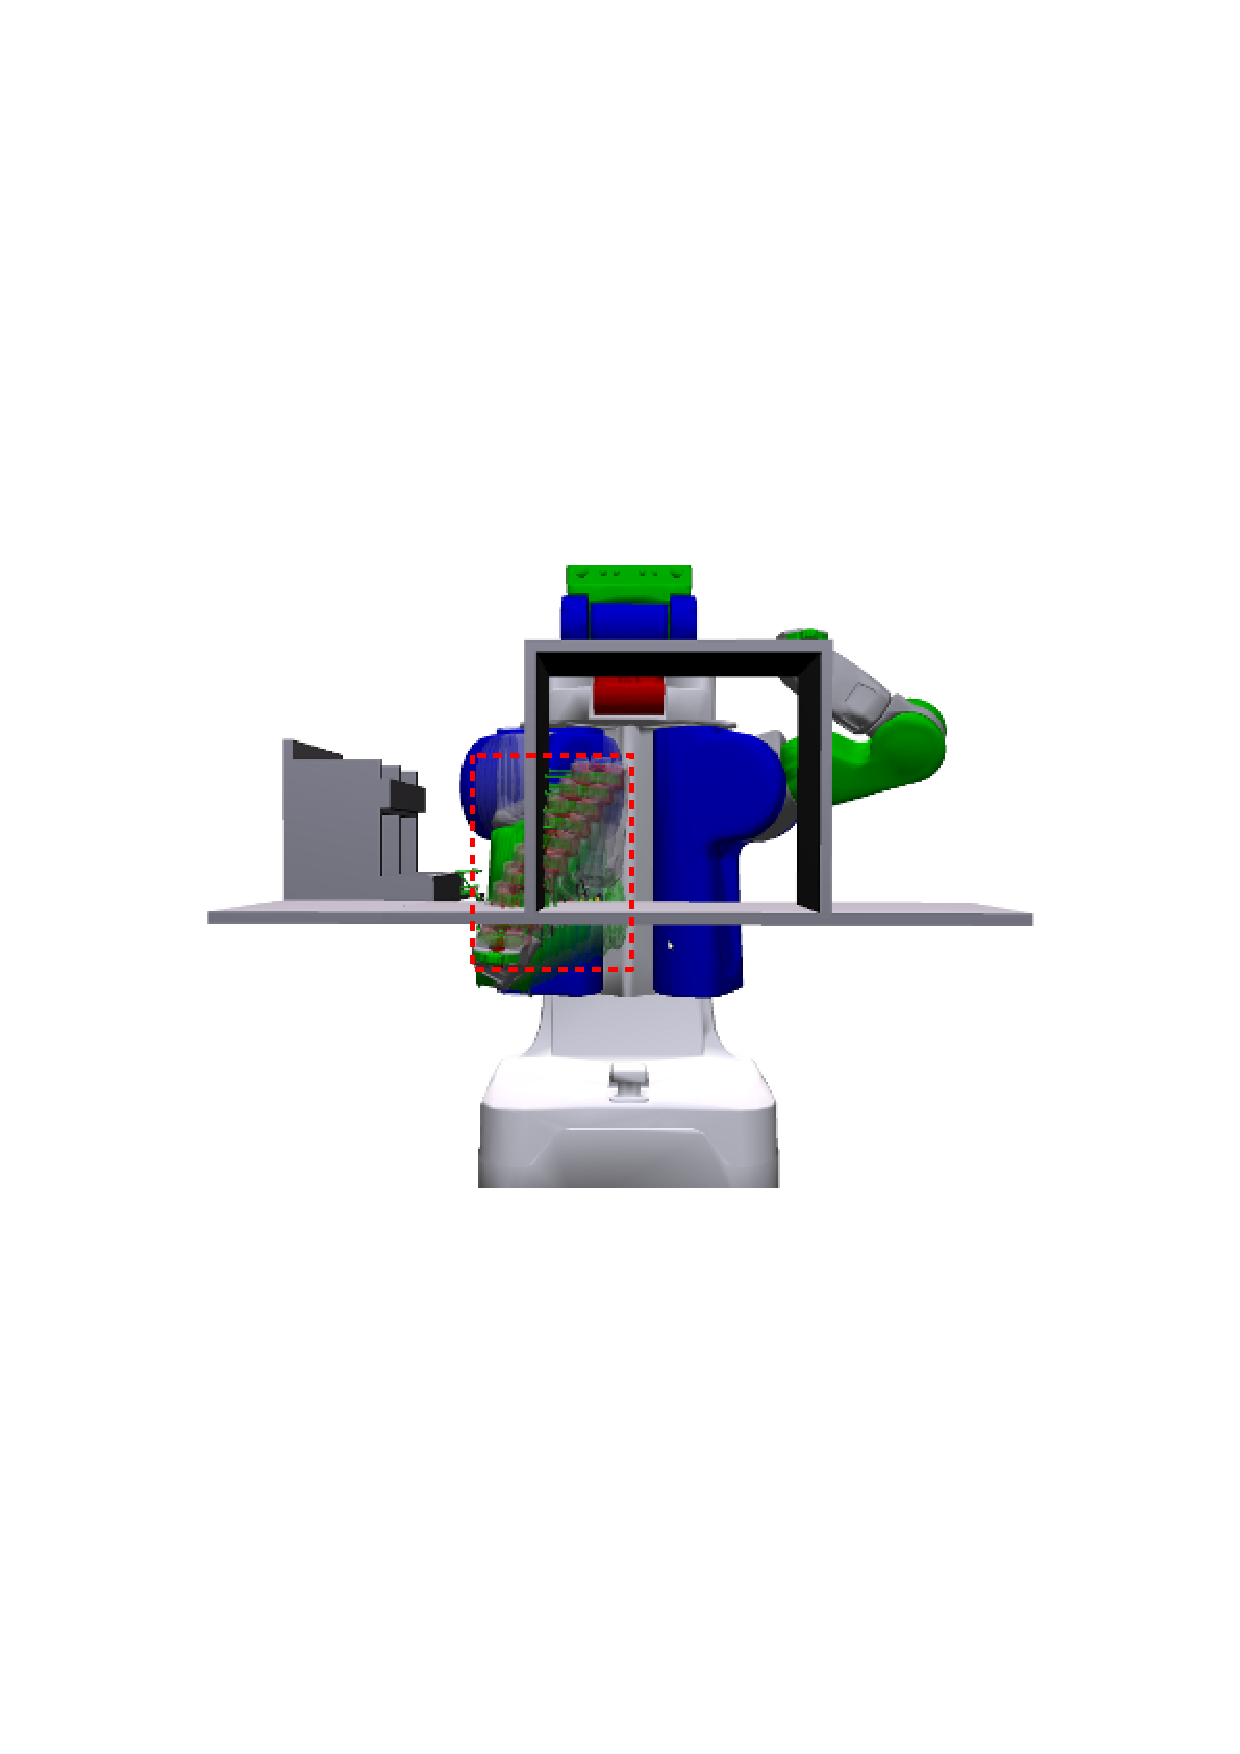
\includegraphics[width=0.38\linewidth]{figure/5.pdf}} \qquad
\subfloat[result path]{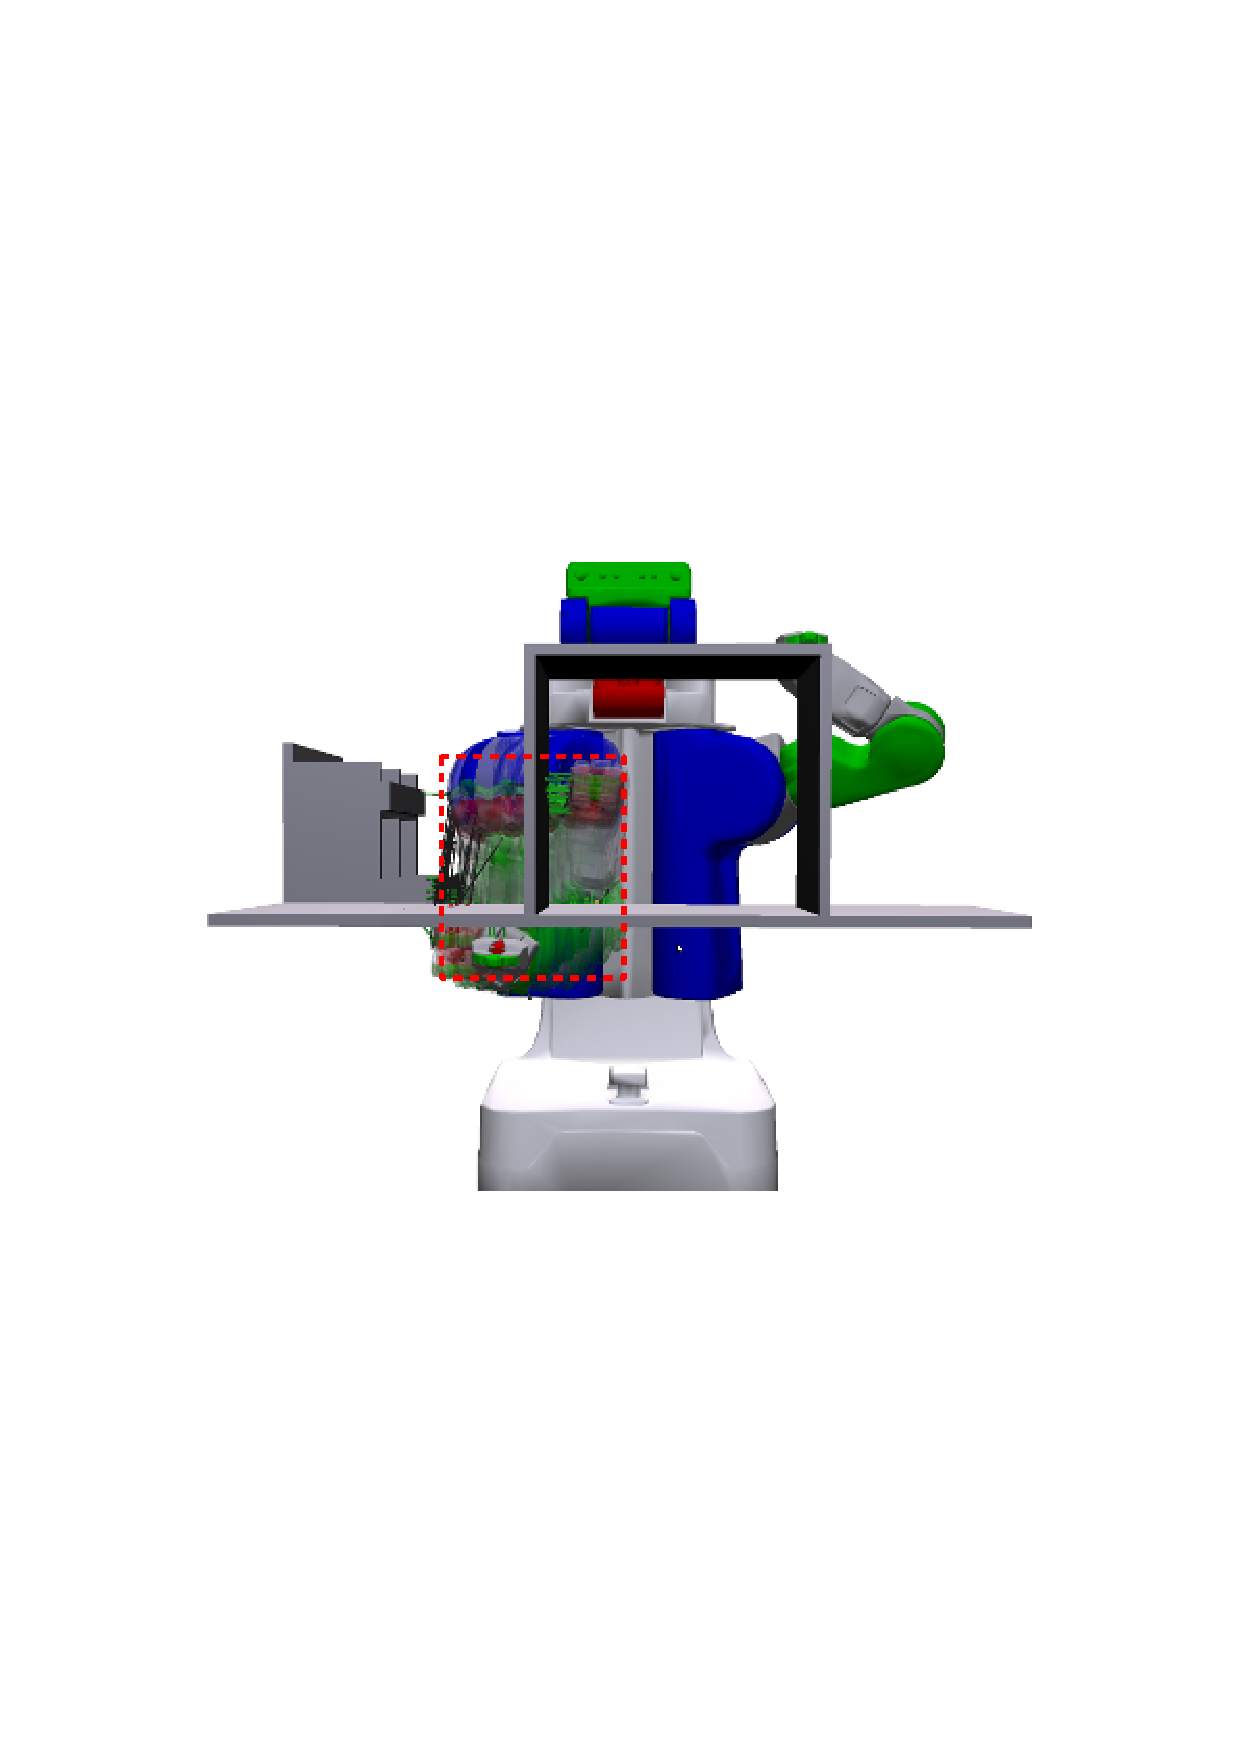
\includegraphics[width=0.38\linewidth]{figure/6.pdf}}
\caption{Failure cases when using the state-of-the-art trajectory optimization method~\cite{Schulman:2013:FLO} for motion planning. (a) shows the initial path for a whole-body planning, which passes through the medial axis of the desk obstacle. (b) is the trajectory optimization outcome, which is stuck in an infeasible condition and the trajectory is pulled apart by virtue of being on both sides of an obstacle. (c) shows the initial path for the arm planning and the collision cannot be resolved in the final trajectory shown in (d). The main difference between trajectories in (c) and (d) is marked by dashed red boxes.}
\label{fig:failexamples}
\end{figure}



We propose a learning-based approach to predict the quality of a trajectory as an initialization to the optimization-based motion planning. Here, a trajectory's quality is measured by whether the optimization problem converges to a collision-free trajectory when using the given trajectory as the initial guess. In other words, the quality is defined in a qualitative manner, i.e. `good' or `bad'.
For the learning algorithm, we first design a set of trajectory features, which are relevant to a trajectory's effectiveness as an initialization. These features are both task-independent and scene-independent, and hence they are transferable among different planning tasks. We use four types of features: (i) spatial signed distance (SSD) vectors for each robot link; (ii) difference between SSD vectors for the same robot link in adjacent trajectory waypoints and for adjacent robot links in the same waypoint; (iii) spherical harmonics transform of SSD vectors; and (iv) features measuring the non-convexity of the constrained optimization problem in the trajectory neighborhood. These features try to capture the obstacle distribution locally around a robot trajectory and thus can be expected to be useful for predicting a trajectory's behavior under a trajectory optimization algorithm. We calcuate these features for a set of randomly selected trajectories for different tasks in various benchmarks. We then run optimization-based motion planning using these trajectories as initial guesses and obtain a labeled dataset. In the dataset, each trajectory is augmented with a `good' or `bad' label according to whether the optimization converges to a collision-free trajectory. With this dataset as the training set, we learn a prediction function for trajectory effectiveness. We evaluate the accuracy of the learned prediction function by counting the ratio of correct predictions for a set of new trajectories on various benchmarks.

\section{Related Work}
\label{sec:related}
Trajectory optimization is an established method in robotics to generate a high quality path from an initial trajectory that may be in-collision or dynamically infeasible. It has also been used as a post-processing phase to remove redundant or jerky motion in trajectories generated by traditional planning algorithms~\cite{Latombe:1991:RMP,Lavalle:2006:PA}. Trajectory optimization works by solving an optimization problem on trajectory space. Many approaches use a spline-based or waypoint-based representation for trajectory and use cost gradient information for minimization, including CHOMP~\cite{Ratliff:2009:CGO}, STOMP~\cite{Kalakrishnan:2011:STOMP} and TrajOpt~\cite{Schulman:2013:FLO}. There is extensive, closely-related work in optimal control, which focuses less on collisions and more on systems with complicated dynamical properties. Some of the most notable work includes differential dynamic programming~\cite{Jacobson:1970:DDP,Atkeson:1994:ULT}, iterative LQR~\cite{Todorvo:2005:iLQG}, approximate inference control~\cite{Toussaint:2009:RTO} and optimization-based control involving contacts~\cite{Mordatch:2012:DCB,Tassa:2012:SSC,Erez:2012:TOD,Posa:2013:DTO}. 

One main challenge of trajectory optimization is its sensitivity to the choice of initial guesses and may get stuck in infeasible local optima, since the collision-free constraint is highly non-convex.

For general non-convex optimization problems, the dependence on initialization is also a well-known challenge. A simple and popular solution is using multiple random initializations to help the algorithms escape from bad local optima. 
In recent work~\cite{Cassioli:2012:MLG} machine learning was used to build the relationship between the starting point of an optimization algorithm and the objective value of the final outcome. The main difference is that our approach is for trajectory optimization, where generating a feasible trajectory is more important than decreasing the absolute cost of the objective function. Moreover, trajectory optimization can exploit workspace heuristics for selecting good initial guesses, and such heuristics are not available in general optimization problems. Another closely related line of work is about trajectory prediction~\cite{Jetchev:2013:FMP}, where learning algorithms are used to predict a good path in a new environment from a database of demonstrated trajectories. The predicted result may not be feasible and hence requires a second step to resolve all violations.

Prior work has considered designing trajectory features for various applications. For example, Bentivegna et al.~\cite{Bentivegna:2006:LST} and Stolle et al.~\cite{Stolle:2007:TPT} represented a library of trajectories by feature vectors for control policy transfer. 
Berenson et al.~\cite{Berenson:2012:RPP} designed several criteria and features to evaluate whether a trajectory from a path library is likely to be reused in a new planning scene after suitable repair operations. Trajectory features are also used to predict class labels of moving objects based on their trajectories~\cite{Lee:2008:TTC}. Moreover, features have been designed to compress trajectory libraries~\cite{Arikan:2006:CMC}. However, all these features only capture properties of a trajectory itself. In contrast, the features proposed in our paper encode the interaction between the trajectory and the surrounding environment, which is critical for predicting how fast a trajectory can be pushed away from the obstacles by a trajectory optimization algorithm.


\section{Problem Definition}
\label{sec:probstatement}

Robotic motion planning problems can be formulated as non-convex optimization problems, i.e., minimize an objective subject to inequality and equality constraints:
\begin{align}
\label{eq:opt}
& \underset{\x}{\text{minimize}}
& & f(\x) \\
& \text{subject to}
& & g_i(\x) \leq 0, \; i = 1, 2, \dots, n_{\text{ieq}} \notag \\
&&& h_i(\x) = 0, \; i = 1, 2, \dots, n_{\text{eq}} \notag
\end{align}
where $f$, $g_i$ and $h_i$ are scalar functions. For planning problems that involve only kinematics and represent the trajectory as a sequence of $T$ waypoints, the optimization variable $\x$ is of the form $\x = \btheta_{1:T}$, where $\btheta_t \in \mathbb{R}^K$ denotes the configuration at the $t$-th waypoint for a system with $K$ degrees of freedom. For problems with dynamics, the optimization variable $\x$ may also include velocities $\dot{\btheta_t}$ and torques ${\bm \tau}_t$.


\begin{figure}[!h]
\centering
\subfloat[]{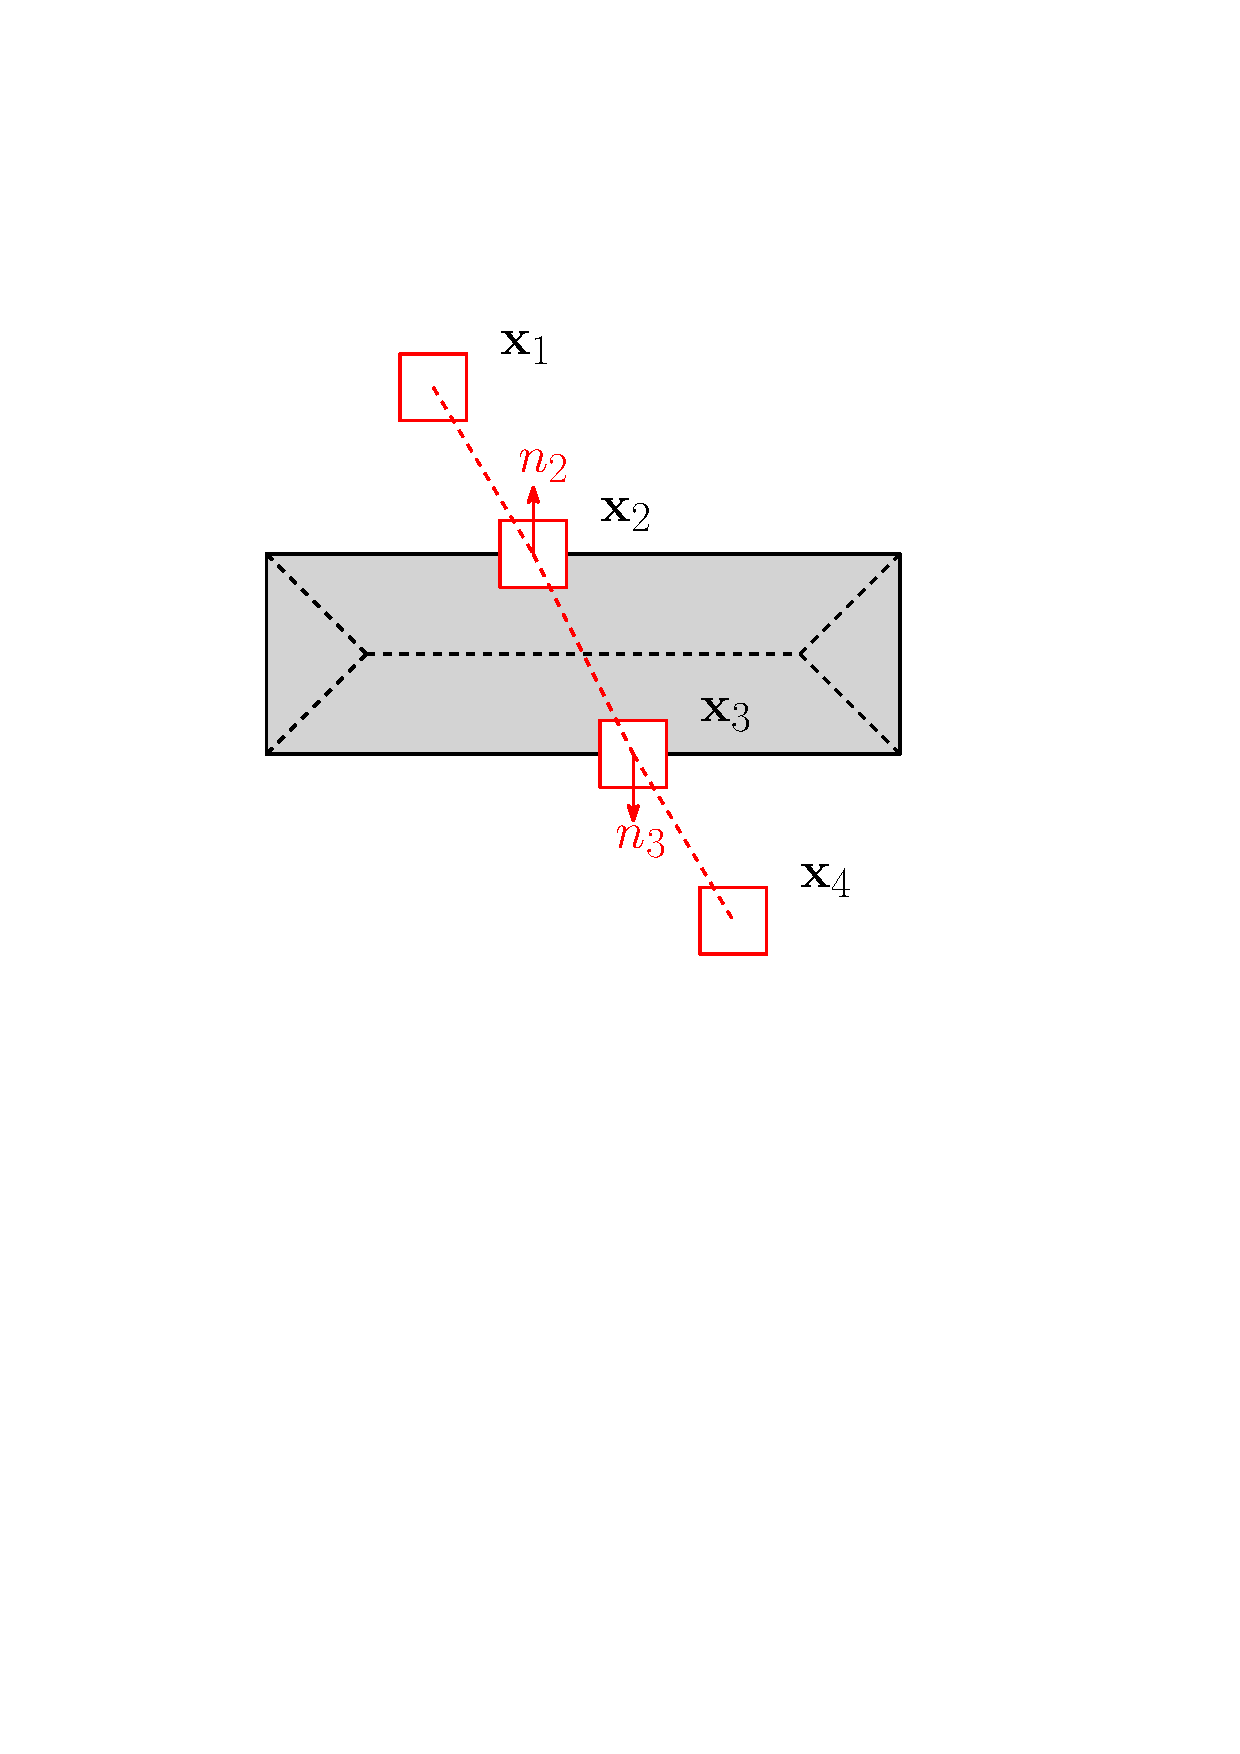
\includegraphics[width=0.34\linewidth]{figure/medial_axis.pdf}} \qquad
\subfloat[]{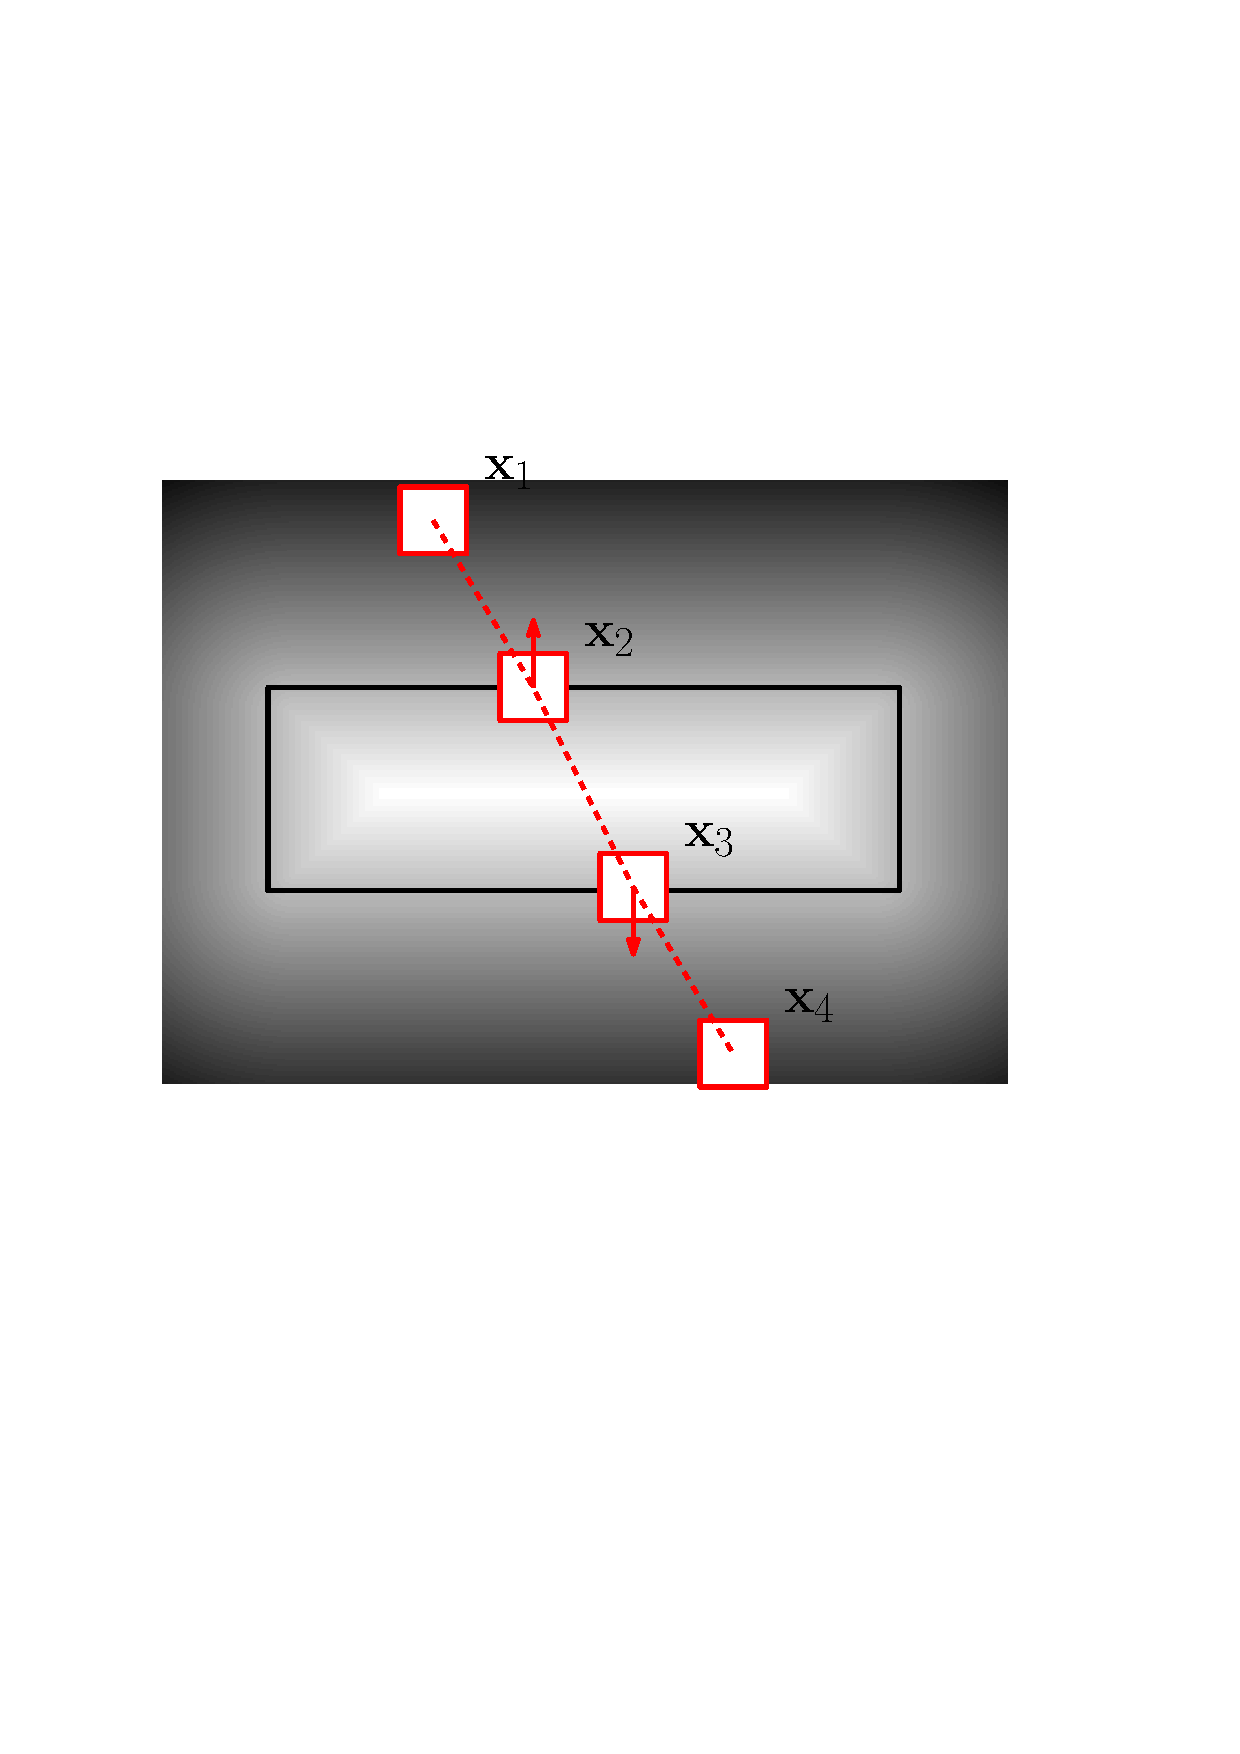
\includegraphics[width=0.44\linewidth]{figure/distance_field.pdf}} \\
\subfloat[]{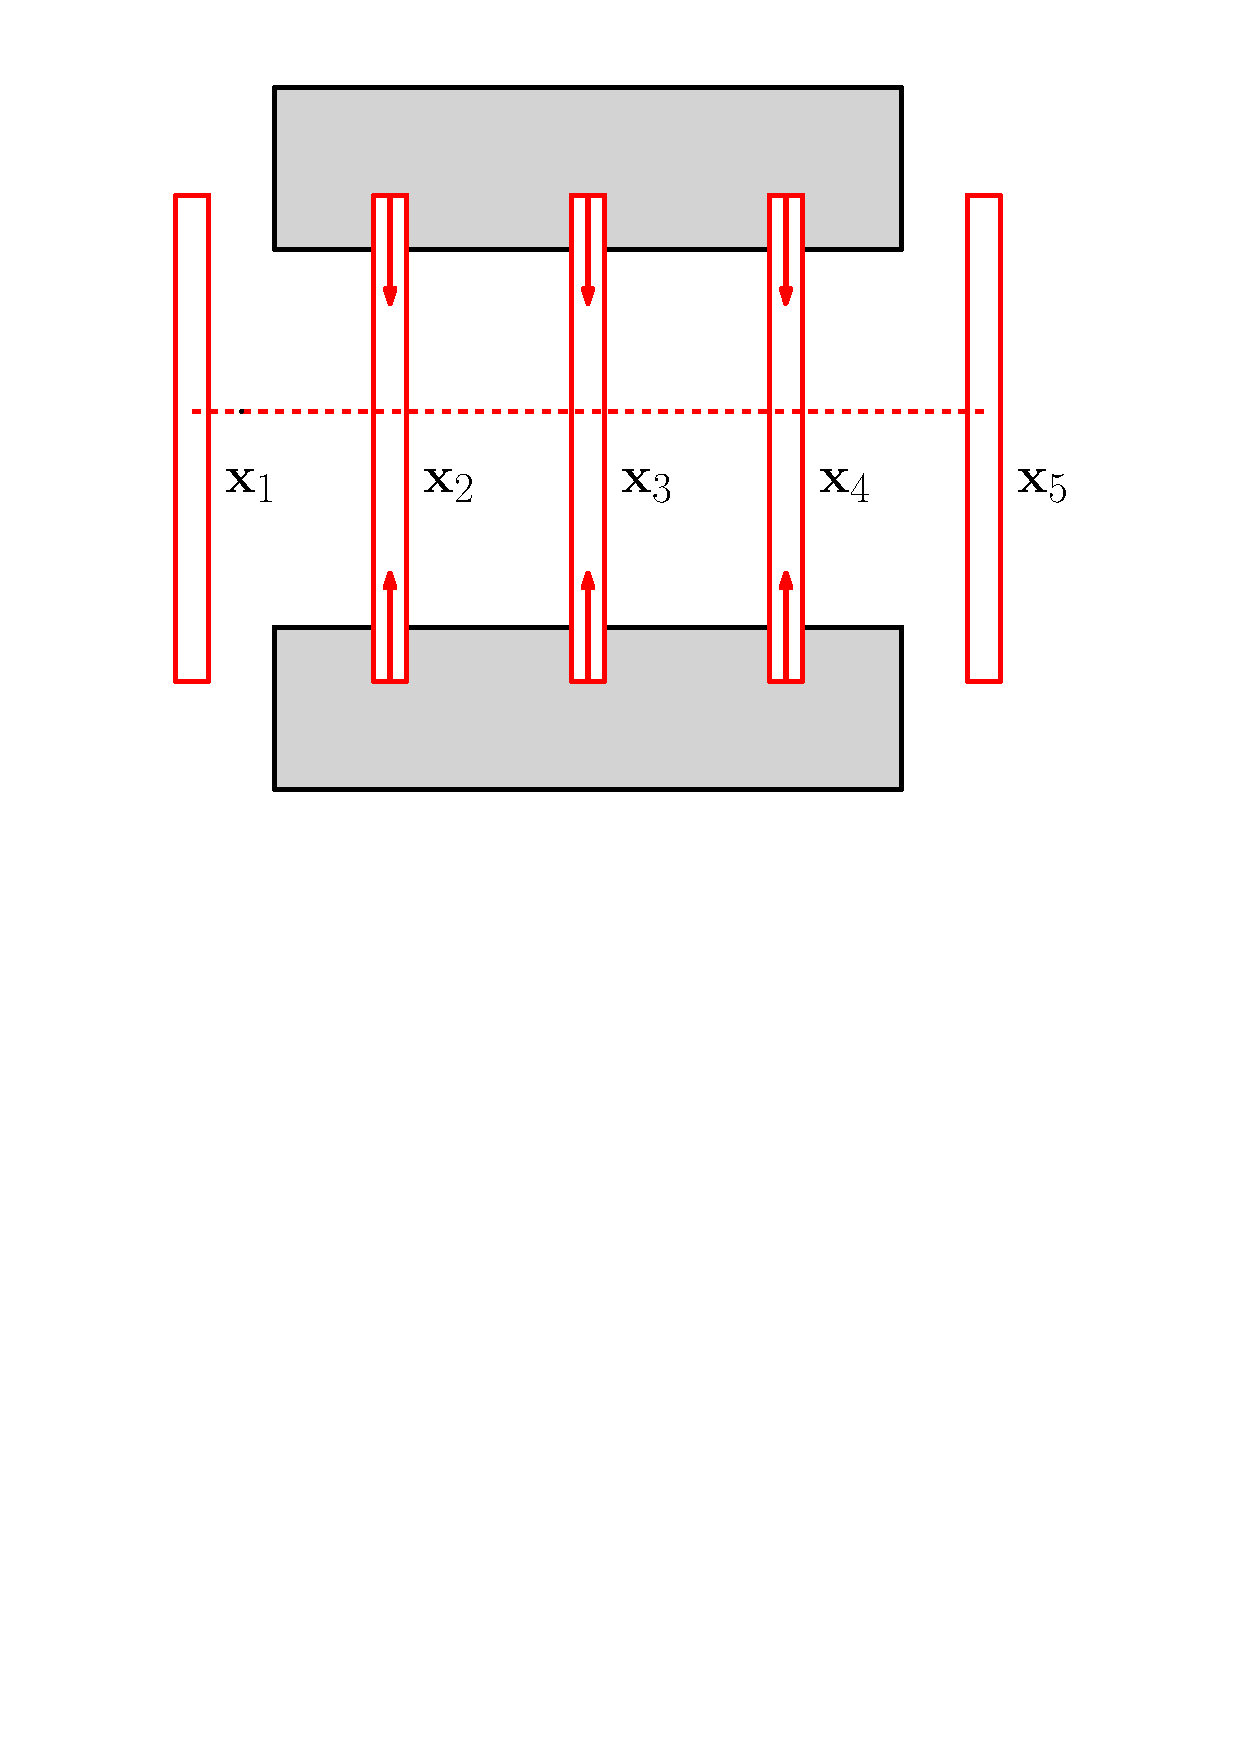
\includegraphics[width=0.38\linewidth]{figure/multiple_obstacle.pdf}} \qquad
\subfloat[]{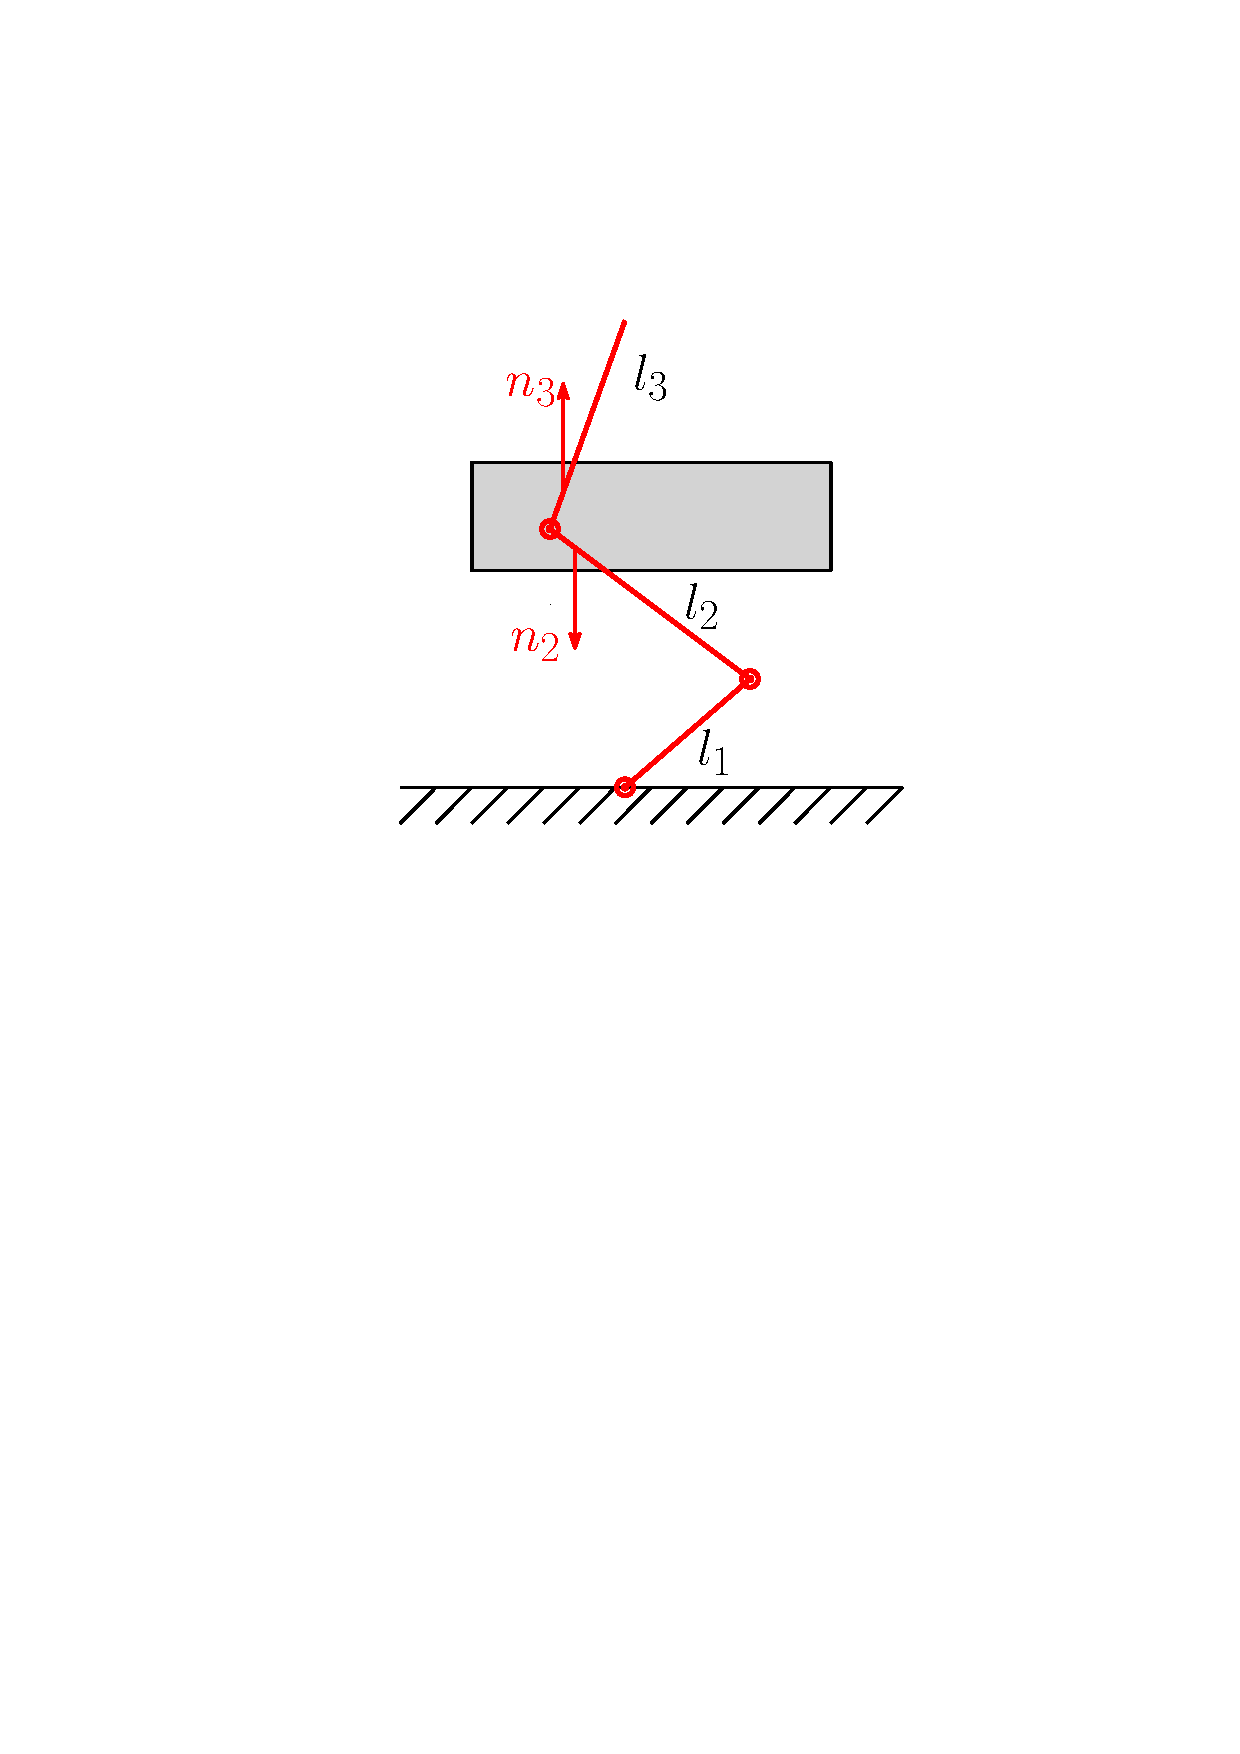
\includegraphics[width=0.38\linewidth]{figure/multiple_link.pdf}}
\caption{Illustration of typical reasons for trajectory optimization to get stuck in local optima that are not collision-free. The gradient based on penetration depth (a) or distance fields (b) may push waypoints in in-consistent directions. When a robot collides simultaneously with multiple obstacles (c), the robot may get stuck in an infeasible local optimum since different obstacles push the robot in different directions. For a robot with multiple links (d), the gradient may result in in-consistent directions for different links. $\mathbf x_i$ in these figures denote different trajectory waypoints.}
\label{fig:badgradient}
\end{figure}


Collision avoidance is one of the most important inequality constraints in motion planning. But it is difficult to be formulated in a closed form and hence is challenging for optimization. Various approximations for collision avoidance constraints have been proposed, including distance fields~\cite{Khatib:1985:ROA, Ratliff:2009:CGO}, penetration depth~\cite{Cameron:1997:CMP}, and swept volume~\cite{Schulman:2013:FLO}. Besides collision avoidance, common inequality constraints include kinematic constraints (e.g., joint limits), kinodynamic constraints (e.g., bounded velocity or acceleration) or dynamic constraints (e.g., dynamic stability constraints). One example of equality constraints is the end-effector pose constraint where the robot must reach a target pose.

The objective function $f(\x)$ is often chosen to be a quadratic form of $\x$. For example, a widely used objective function for kinematic planning is $f(\btheta_{1:T}) = \sum_{t=1}^T \|\btheta_{t+1} - \btheta_{t}\|^2$, which encourages minimum-length or smoothness in the final outcome~\cite{Schulman:2013:FLO,Ratliff:2009:CGO}.


Trajectory optimization is a challenging non-convex problem, and many approaches have been presented to solve it effectively. Among them are sequential convex optimization~\cite{Schulman:2013:FLO}, covariant Hamiltonian optimization~\cite{Ratliff:2009:CGO}, and stochastic optimization~\cite{Kalakrishnan:2011:STOMP}. However, given an initial trajectory that contains collisions, none of these methods are guaranteed to find a collision-free solution due to the non-convex constraints in the optimization. Figure~\ref{fig:badgradient} shows some scenarios illustrating how trajectory optimization tends to get stuck in local optima that are not collision-free. 


It is an on-going line of research to reshape the non-convex optimization formulations to improve their performance. In this paper we consider the following complimentary problem: Given a trajectory optimization approach, how to predict whether an initialization will result in a collision-free solution or not. 
Such predictive capabilities would enable selecting a good initial trajectory for motion planning so that trajectory optimization is likely to converge to a collision-free local optimum. Such information can also be used to improve the performance of trajectory optimization being run in parallel for multiple initializations: For each solution sequence starting with a different initial guess, we can stop bad solution sequences early enough and focus computational budgets on solution sequences that potentially can converge to good outcomes.


\subsection{Outline of Proposed Approach}
The problem to predict whether a given trajectory is a good or bad initial guess for a trajectory optimization algorithm can be formalized as a two-class classification problem. In fact, a trajectory is good if and only if it locates in the basin of attraction of a local optimum that is collision-free.

For the classification problem, we first design trajectory features that are potentially useful to distinguish good and bad initializations. The features extracted from a trajectory $\btheta_{1:T}$ are denoted as a vector $\fsym = E(\btheta_{1:T})$, where $E(\cdot)$ is the extraction function. For each trajectory, we use a binary variable $y$ to denote whether the trajectory optimization succeeds ($y = 1$, a good initial guess) or fails ($y = 0$, a bad initial guess). 


Given a set of $N$ trajectories, we build a training set $\{\fsym_i, y_i\}_{i=1}^N$. Based on the data set, we learn a classifier $C(\fsym) $, which is the predictor for a trajectory's effectiveness. Given a new trajectory as input, $C(\cdot)$ will provide its qualitative evaluation (good or bad) as output. The learned predictor $C(\cdot)$ can depend on the planning methods, because different optimization approaches may differ in for which initial trajectories they end up finding feasible solutions.  However, our learning method is general and does not depend on the type of trajectory optimization method.


\section{Predicting Initialization Effectiveness for Trajectory Optimization}
\label{sec:predict}
In this section, we design trajectory features to distinguish good and bad initializations and use the extracted features for predicting the effectiveness of a new trajectory.


Before extracting features from a trajectory, we first perform re-sampling on it so that waypoints are uniformly distributed between two end-points.
We perform this pre-processing based on what was pointed out by Ratliff et al.~\cite{Ratliff:2009:CGO}: the objective function should be invariant to the re-parameterization of the trajectory so that the gradient will pull a trajectory out of obstacles instead of encouraging it to quickly jump through obstacles. Some recent work such as~\cite{Schulman:2013:FLO} handles the `jumping through problem' in a completely different way, but in practice, it is observed that a re-sampling pre-processing can still result in better convergence. 
The re-sampling process removes some the parameterization-dependent differences between trajectories and hence makes it easier to compare them. After re-sampling, each trajectory has $T$ waypoints. This also results in fixed-length feature vectors.


\subsection{Background: Signed Distances}
We design features to encode the obstacle distribution locally around a trajectory, as such information is closely related with a trajectory's effectiveness. Intuitively speaking, if a trajectory is deep inside the obstacles, it is less likely to be pushed out of them; whereas if it is mostly outside the obstacles, it should converge to a collision-free solution. To quantify the obstacle distribution surrounding a trajectory, we use signed distances and normals, which are used in previous trajectory optimization algorithms such as~\cite{Schulman:2013:FLO}. Informally, the signed distance between two objects is the length of the smallest translation that puts them in contact; the signed normal is the direction of such translation. The signed distance can be efficiently computed for convex objects using GJK algorithm~\cite{Gilbert:1988:GJK} and EPA algorithm~\cite{Bergen:2001:EPA}.   For use with non-convex objects, these objects can be represented as a set of convex objects together making up the original non-convex object.


\subsection{Feature I: Spatial Signed Distance Vectors}
Based on the signed distances formulation, a natural choice for designing trajectory feature vector is to collect signed distances and normals between all pairs of robot links and environment obstacles, for each waypoint in the trajectory. More formally, given a robot with $n$ links $\mathcal A_i$ in an environment with $m$ obstacles $\mathcal B_j$, the feature vector would be $\fsd = \{\text{sd}_{i,j,t}, \mathbf n_{i,j,t}\}_{1\leq i \leq n, 1\leq j \leq m, 1\leq t \leq T}$, where $\text{sd}_{i,j,t} = \text{sd}(\mathcal A_i(t), \mathcal B_j)$ is the signed distance value between $\mathcal A_i$ and $\mathcal B_j$ at waypoint $\btheta_t$, and $\mathbf n_{i,j,t}$ is the corresponding normal. This feature vector is of dimension $4\times m \times n \times T$ and provides a complete description for the obstacle distribution around the trajectory. However, the dimension of this feature depends on $m$, the number of obstacles in the environment, which makes this feature not transferable among different environments. Moreover, in many real-world systems, there may be a large number of obstacles (e.g., the obstacles from sensor data are usually represented as thousands of boxes~\cite{Sucan:2010:CPT}). This would result in a long feature vector and brings challenges for both data storage and the following learning procedure. Thus we propose to summarize this information in a more compact manner that lends itself better to generalization.

\begin{figure}[!h]
\centering
\subfloat[]{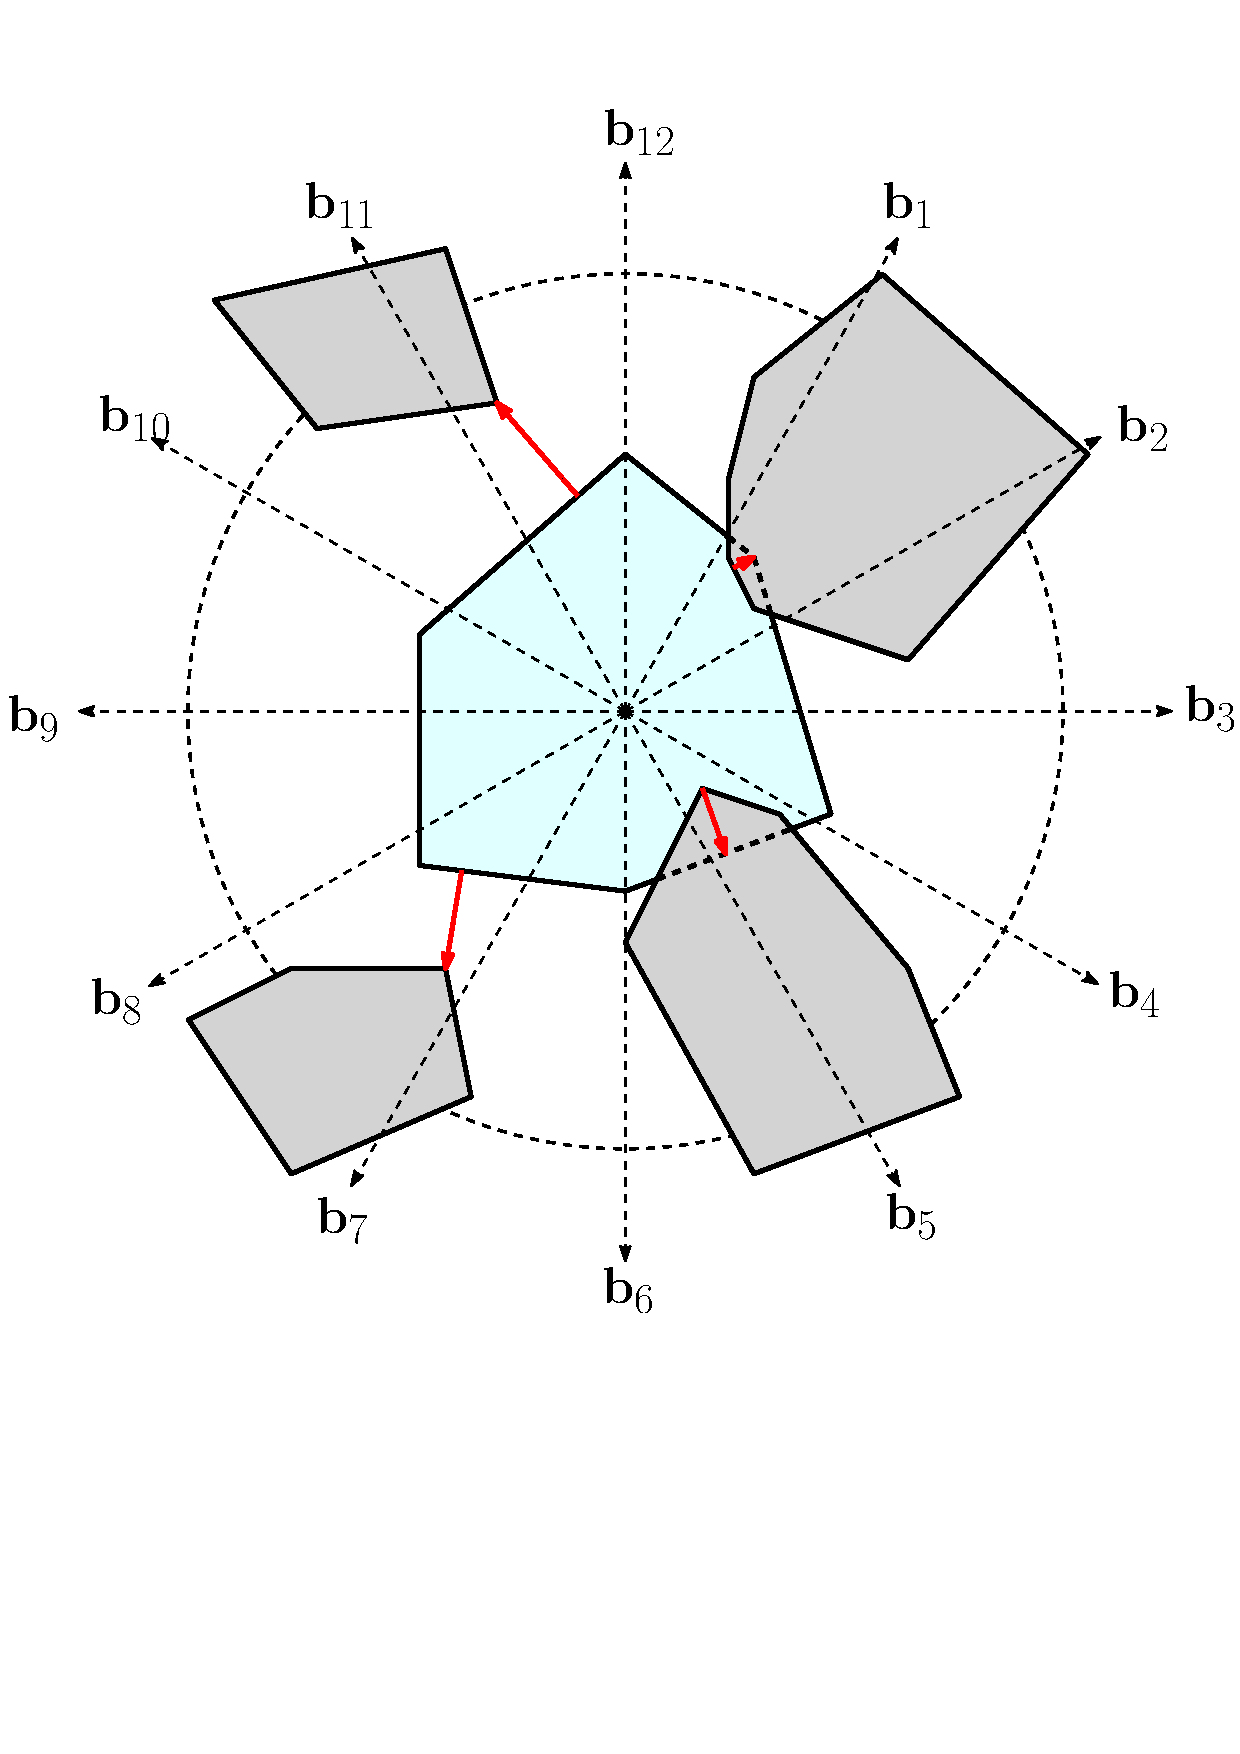
\includegraphics[width=0.52\linewidth]{figure/penetration_encode.pdf}}
\subfloat[]{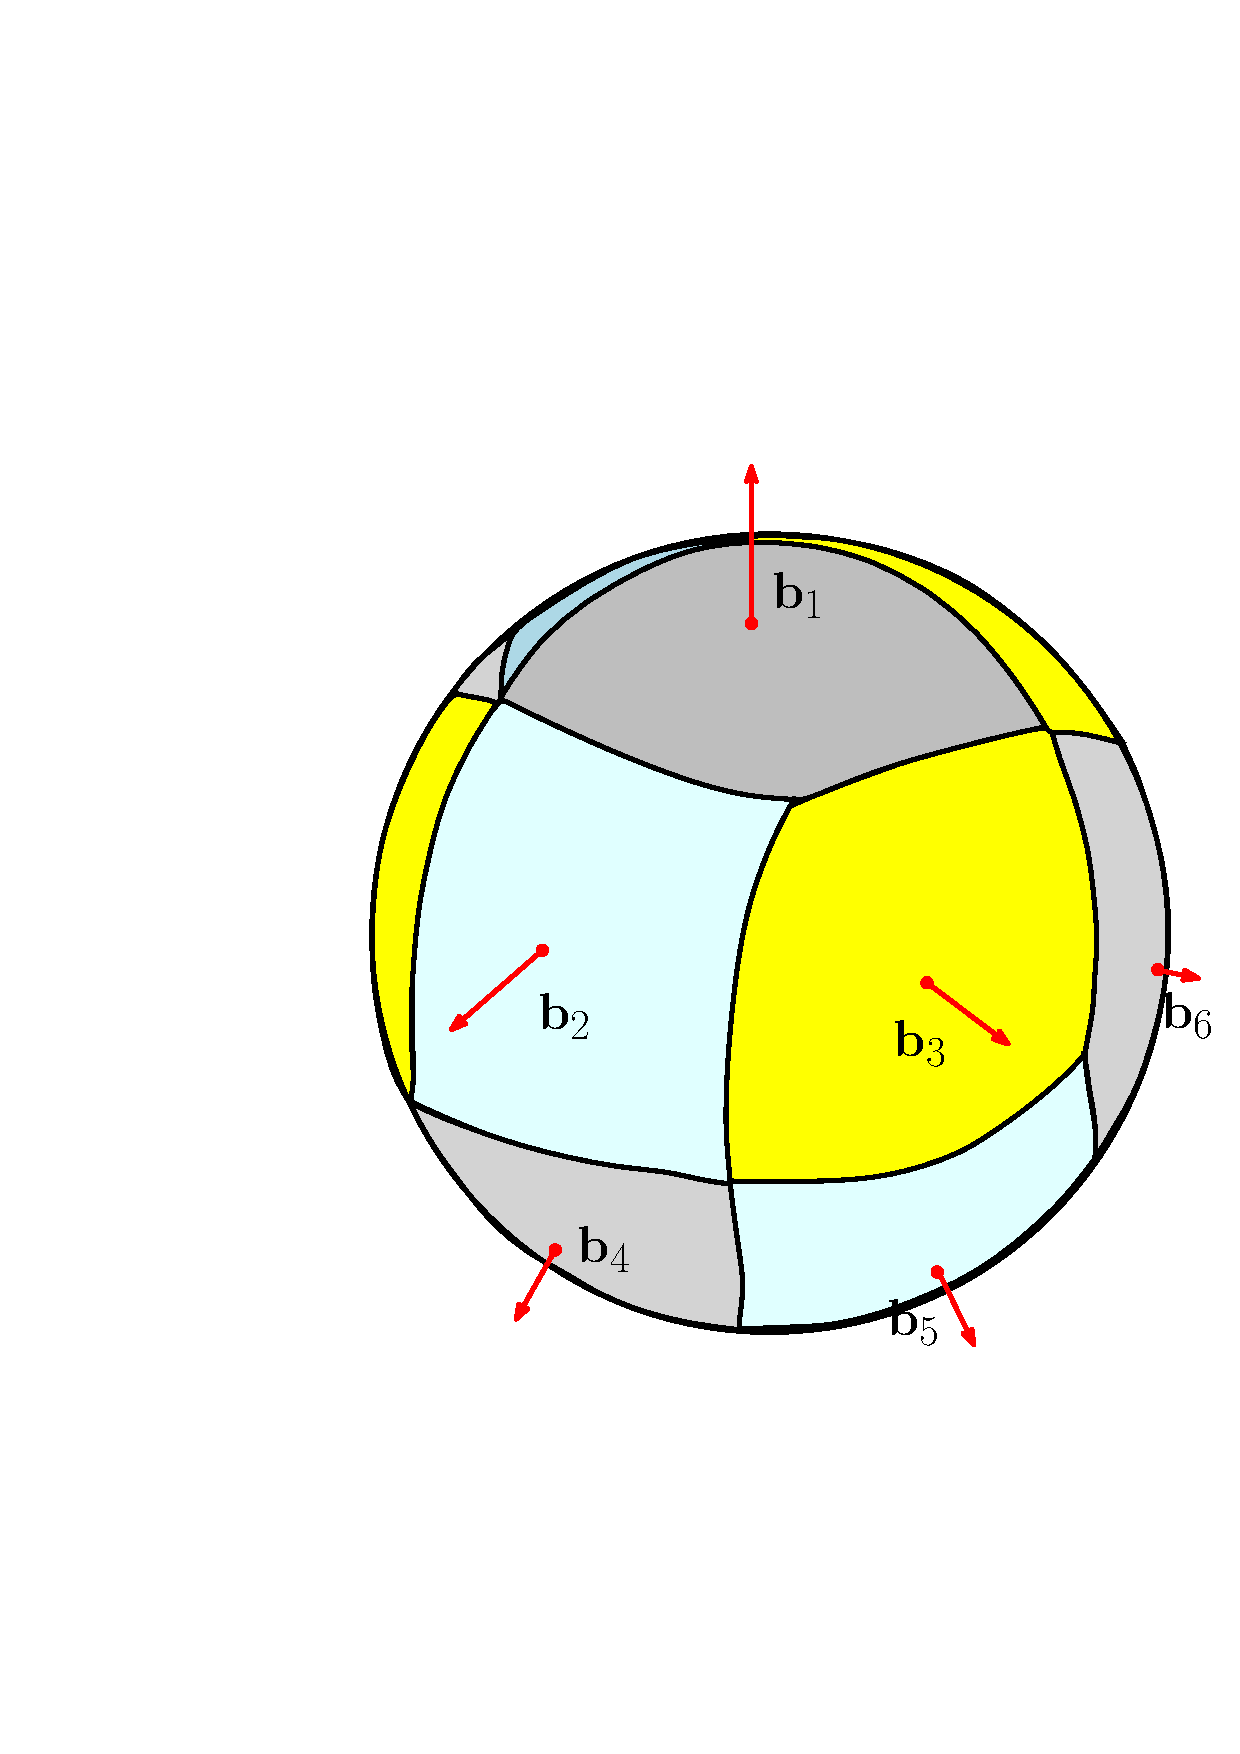
\includegraphics[width=0.47\linewidth]{figure/discrete_directions.pdf}}
\caption{Spatial signed distance vectors: (a) shows a 2D example about SSD vector generation. The surrounding space around a robot link (the cyan color part) is uniformly divided by a spatial vector dictionary with $12$ directions $\{\mathbf b_1, ..., \mathbf b_{12}\}$. The signed distance value $\text{sd}_j$ between the robot and the $j$-th obstacle (the grey part) is then accumulated toward a direction $\mathbf b_k$, which has the smallest angle with the corresponding signed distance normal $\mathbf n_j$, i.e., with the smallest $|\mathbf n_j \cdot \mathbf b_k|$. (b) In 3D case, we use the approach introduced in~\cite{Yershova:2010:GUI} to generate dictionary vectors that make equisurface partition on a sphere surface. }
\label{fig:trajectoryfeaturePD}
\end{figure}

Our solution is to re-organize the signed distances and normals into a new form called the Spatial Signed Distance (SSD) vectors. We illustrate the basic idea of SSD via a 2D example in Figure~\ref{fig:trajectoryfeaturePD}(a). We first partition the space around a robot link using a dictionary of direction vectors $D = \{\mathbf b_1, ..., \mathbf b_M\}$.  For the 3D case, we generate the direction dictionary using the approach introduced in~\cite{Yershova:2010:GUI}, which computes a uniform deterministic sequence of samples over $S^2$ (as shown in Figure~\ref{fig:trajectoryfeaturePD}(b)) using a specific multi-resolution grid structure.  This partitions the sphere surface into bins of the same size.

Given the signed distances and normals between the robot link and all the obstacles in the environment, we accumulate the signed distances along these discretized prototype directions in dictionary $D$ and the result is a $M$-dimensional vector $\fssd$. The $k$-th element of $\fssd$ is denoted as $\fssd[k]$, which summarizes signed distances along direction $\mathbf b_k$. If $\fssd[k]$ is positive, then the link still has some distance from the obstacle and is safe; if $\fssd[k]$ is negative, then the link will go deeper inside the obstacle when being pushed in this direction and hence should be pushed in other directions. 


The algorithm to compute $\fssd$ based on signed distance information is shown in Figure~4. First, each element in $\fssd$ is initialized by a default value $R > 0$, which defines the size of the local neighborhood around the link. We set $R$ to be the robot link's bounding radius; this implies that a large object would have a larger local neighborhood. Next, suppose the $j$-th obstacle's signed distance to the robot link is $\text{sd}_j$ and the corresponding normal is $\mathbf n_j$. We first find the dictionary direction $\mathbf b_k$ which has the smallest angle with $\mathbf n_j$, i.e., quantizing $\mathbf n_j$ to the prototype direction $\mathbf b_k$ with the smallest $|\mathbf n_j \cdot \mathbf b_k|$. Next, we merge $\text{sd}_j$ with the existing value in $\fssd[k]$. If both $\text{sd}_j$ and $\fssd[k]$ are negative, i.e., a new penetration is detected in a direction where the penetration was detected before, we add $\text{sd}_j$ onto $\fssd[k]$ to give a large penalty for such in-collision case. For other cases, we update $\fssd[k]$ by $\text{sd}_j$ if $\fssd[k]$'s current value is larger than $\text{sd}_j$. In other words, $\fssd[k]$ is with the signed distance value of the closest obstacle. If $\fssd[k]$ remains $R$ after the computation, this means that no penetration is detected within the given link's neighborhood along direction $\mathbf b_k$. In this way, we summarize the obstacle distribution information around a robot link into a length-$M$ SSD vector.

\begin{figure}[!h]
\textbf{Input}: Signed distance values $\text{sd}_j$ and normals $\mathbf n_j$ between the robot link and the $m$ obstacles in the environment; The spatial vector dictionary of size $M$: $D = \{\mathbf b_1, ..., \mathbf b_M\}$\\
\textbf{Output}: Spatial signed distance vector $\fssd$
\begin{algorithmic}[1]
\State{Initialize $\fssd$ as a dimension-$M$ vector with default value $R$;}
\For{$j \leftarrow 1$ to $m$}
	\State{Find $\mathbf b_k$ in $D$ where $|\mathbf b_k \cdot \mathbf n_j|$ is the smallest;}
	\If{$\text{sd}_j < 0$ \text{and} $\fssd[k] < 0$}
		\State{$\fssd[k] \leftarrow \fssd[k] + \text{sd}_j$;}
	\Else
		\State{$\fssd[k] \leftarrow \min(\fssd[k], \text{sd}_j)$;}
	\EndIf
\EndFor
\end{algorithmic}
\label{algo:SSD}
\caption{SSD vector generation for one robot link at a trajectory waypoint}
\end{figure}


After computing SSD vectors for all links belonging to all trajectory waypoints, we concatenate them together into the SSD feature vector for the entire trajectory, which is of dimension $n\times M \times T$ and is also denoted as $\fssd$. For environments with many obstacles, $M \ll m$ and therefore $\fssd$ is more compact than $\fsd$.



\subsection{Feature II: Difference between Spatial Signed Distance Vectors}
The spatial signed distance vector provides a description of the obstacle distribution around the trajectory on a per link basis. However, as we mentioned in Section~\ref{sec:probstatement}, whether the signed distance normal is consistent between adjacent links or adjacent waypoints in an initial trajectory is also important for the convergence of a trajectory optimization algorithm. Thus, we include features to measure the consistency between two spatial signed distance feature vectors. Given two vectors $\fssd^a$ and $\fssd^b$, we evaluate their consistency using their dot-product $\fssd^a \cdot \fssd^b$. This dot-product has a larger value when $\fssd^a[k]$ and $\fssd^b[k]$ are of the same sign for all $k$. And it has a smaller value when some $\fssd^a[k]$ and $\fssd^b[k]$ are of the opposite sign, i.e., the signed distance normals are not consistent in direction $\mathbf b_k$. We compute dot-product between SSD vectors of the same link in adjacent waypoints and between adjacent links in the same waypoint. We collect all these results relating to consistency in the signed distances in a feature vector denoted by $\fcon$.

\subsection{Feature III: Spherical Harmonics Spatial Feature}
The spatial signed distance feature is not rotation-invariant.
As a result when, for example, both the environment and the trajectory are rotated by a given angle, the feature vector will be completely different.  This could affect its generalization capability. Another example is when the environment is symmetric (such as Figure~\ref{fig:benchmarks1}(c)).  Overall, the lack of rotation-invariance in the feature may decrease the prediction accuracy of the learning algorithm.


As shown in Figure~\ref{fig:trajectoryfeaturePD}(a), the spatial signed distance feature is a function defined on a sphere around a robot link. To represent the feature in a rotation-invariant manner, we utilize spherical harmonics. The same idea has been used in various applications, including computer vision~\cite{Frome:2004:ROR} and graphics~\cite{Kazhdan:2003:RIS}.

The theory of spherical harmonics says that any spherical function $s(\theta, \phi)$ can be expressed as a sum of complex spherical harmonic basis functions $Y_l^m$: 
\begin{equation}
s(\theta, \phi) = \sum_{l=1}^{\infty} \sum_{m=-l}^{l} a_l^m Y_l^m(\theta, \phi).
\end{equation}
The amplitudes of the harmonic coefficients $\|a_l^m\|$ are invariant to any rotation in the azimuthal direction. Moreover, the amplitude of $s_l$, the $l$-th frequency component of the function $s$, is rotation-invariant under any rotations, where $s_l = \sum_{m=-l}^{l}a_l^m Y_l^m(\theta, \phi)$. The magnitude of $s_l$ can also be computed based on $a_l^m$: $\|s_l\|^2 = \sum_{m=-l}^l \|a_l^m\|^2$. We use $\|s_l\|$ as features in 3D benchmarks. In 2D case, we use $\|a_l^m\|$ as features since only azimuthal rotation is allowed in 2D and $\|a_l^m\|$ can provide richer information. Similar to previous work~\cite{Frome:2004:ROR,Kazhdan:2003:RIS}, we choose a bandwidth $b$ and store only $b$ lowest-frequency components in our spherical harmonics feature $\fsht$. More formally, the feature is defined as $\fsht = \{\|s_l\|\}$ in 3D and $\fsht = \{\|a_l^m\|\}$ in 2D, where $m = 0,...,l$ and $l = 0,...,b$.


\subsection{Feature IV: Convexity Features}
As another category of features, we also measure the local convexity of the trajectory optimization problem around the initial trajectory. 
The optimization problem formalized in Equation~\ref{eq:opt} usually involves non-convex objective and constraints. In trajectory optimization algorithms, these non-convex terms are approximated by convex functions in each iteration of the optimization. The convexity features quantify how close the approximations are in such `convexify' steps.

We first compute Hessian matrices of the objective and constraint functions at the trajectory. Next, to measure the local non-convexity of the optimization problem, we compute the following features based on the eigenvalues of the Hessian matrices: (i) the minimum eigenvalue; (ii) the sum of negative eigenvalues; (iii) the maximum eigenvalue; (iv) the sum of all eigenvalues. We compute these four statistics for each objective and constraint function, and generate a total of $4 times T \times (1 + n_{\text{ieq}} + n_{\text{eq}})$ convexity features, which are collected in a feature vector denoted as $\fconv$.


\subsection{Trajectory Evaluation and Effectiveness Prediction}
To evaluate whether a trajectory is `good' or `bad' as the initial guess for the optimization, currently we use two simple criteria: a trajectory is justified as a `good' initialization if the optimization algorithm converges and the final outcome does not violate any constraints. 

Given a set of trajectories with their features and evaluation results, we can use any two-class classification algorithm to learn a classifier for the trajectory. As the dimension of our trajectory feature is high (larger than $200$), we choose the linear support vector machine~\cite{Cortes:1995:SN} as the classifier due to its simplicity and efficiency.

\section{Experiment and Evaluation}
\label{sec:experiment}
We experimentally evaluate the trajectory features that we designed and demonstrate the accuracy of our effectiveness prediction approach on various 2D and 3D benchmarks, as shown in Figure~\ref{fig:benchmarks1},~\ref{fig:benchmarks2} and~\ref{fig:benchmarks3}. The trajectory optimization algorithm we used in the experiment is TrajOpt~\cite{Schulman:2013:FLO}, which is one of the state-of-the-art trajectory optimization algorithms.

\subsection{Experiment Setting}
For each benchmark, we have a pre-defined set of task settings (the initial and goal configurations) as seed tasks. For PR2 benchmarks, we use the $198$ arm planning problems and $96$ full-body problems used in TrajOpt~\cite{Schulman:2013:FLO}. For dubins car benchmarks, we manually select a set of initial-goal configurations that should have feasible solutions. Next, we perturb the initial and goal configurations around these seed tasks to generate more random tasks. We filter out the invalid tasks where the initial or goal configurations are in-collision. We also remove the trivial cases where the linear interpolation between initial and goal is collision-free. We did not randomly select tasks in the entire configuration space because this will incorrectly bias the classifier toward tasks that will hardly happen in real world robotics applications.


Given one planning task, we first generate a trajectory which is a simple linear interpolation between the initial and goal configurations. Next, we perform random perturbation of the trajectory waypoints and generate more random trajectories. For each of these trajectories, we run the trajectory optimization algorithm using it as the initial guess. When the optimization stops, we will obtain a sequence of trajectories. These intermediate trajectories can also be used as initializer and they would all have the same effectiveness label as the actual initial guess. As a result, if the optimization converges and the final outcome is feasible, we evaluate the given initial trajectory and all intermediate trajectories as `good' initializations. Otherwise we evaluate all of them as `bad'. Finally, we extract features for all these labeled trajectories and add them into the dataset. In this way, we generate more than $10,000$ trajectories for each planning benchmark. For each benchmark, we use half of the data for training a classifier and the rest for testing experiments. When splitting training and test sets, we make sure that trajectories corresponding to the same task are assigned into the same set, in order to guarantee that the test set is independent of the training set. In Figure~\ref{fig:features}, we visualize the features of two trajectories from different benchmarks. Except $\fconv$, all these features can be computed in less than 10 milleseconds per trajectory. $\fconv$ is more expensive (about 8 seconds) since it is time consuming to compute a trajectory's Hessian matrix numerically.

\subsection{Effectiveness Prediction on Same Benchmarks}
We first show the prediction accuracy when using a classifier learned on one benchmark to predict the effectiveness of trajectories in the same benchmark but for different tasks. The results are shown in Table~\ref{tab:result}, where we compare the baseline accuracy and the accuracy when different combinations of features are used to train a classifier. From the results, we observe that the learned classifiers provide accuracy significantly higher than the baseline (which simply predicts according to the majority label in the training set). However, the peak accuracy may be achieved by different combination of features on different benchmarks.

\subsection{Effectiveness Prediction on Different Benchmarks}
A more challenging test is to check whether a classifier learned on one benchmark is able to correctly predict effectiveness for trajectories from other benchmarks. For this test, we only obtain partial success: We indeed observe several successful transfers among different benchmarks as shown in Table~\ref{tab:result2}. However, in most cases, the prediction accuracy is low when transferring between different benchmarks.

There are several reasons for the poor transfer performance of the current prediction algorithm. First, our current feature design only considers the spatial information locally around the trajectory and does not take into account the global description about the environment, which has been proved to be helpful for trajectory transferring between different environments~\cite{Jetchev:2013:FMP}. For instance, the classifier learned on squared-dubin in Figure~\ref{fig:benchmarks1}(c) can be successfully transferred to jagged-dubin in Figure~\ref{fig:benchmarks1}(a) because the environments are similar. The transfer to gap-dubin in Figure~\ref{fig:benchmarks1}(b) is difficult because the existence of the narrow gap, which does not exist in squared-dubin or jagged dubin benchmark. Second, a high-DOF robot may use different part of DOFs in different scenarios; this results in different trajectory distributions on different benchmarks. Hence, we need more trajectory data from various scenarios and tasks, in order to completely cover the trajectory space. Finally, the rotation-invariance of features is also important for transferring. From the successful case shown in Table~\ref{tab:result2}, we observe that the feature combination $\fcon+\fsht$ behaves the best in transferring, and both of them are rotation-invariant features. 

\begin{figure*}[t]
\centering
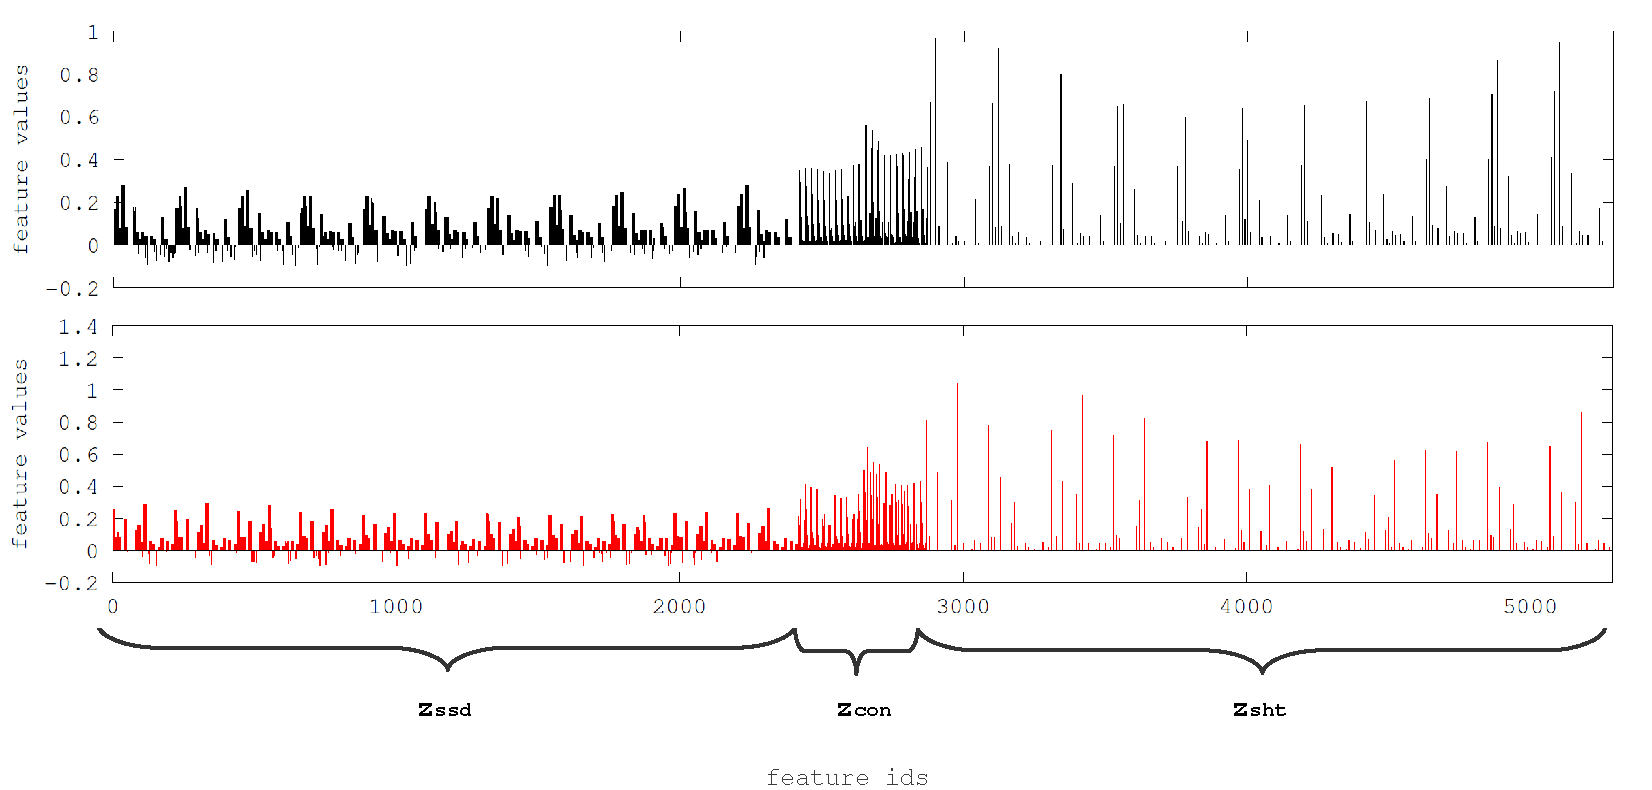
\includegraphics[width=0.8\linewidth]{figure/features.pdf}
\caption{Features for two different trajectories in the bookshelf benchmark. Rough periods appears for all the three sub-features $\fssd$, $\fcon$ and $\fsht$, because these features are computed for each trajectory waypoint.}
\label{fig:features}
\end{figure*}

\begin{table*}[tbp]
\rowcolors{1}{gray!25}{}
\centering
\begin{tabular}{|c|r|r|r|r|r|r|r|r|r|}
\hline 
 & baseline & ${\bf z}_\textrm{conv} +\fssd+\fcon+\fsht$  & $\fssd+\fcon+\fsht$ & $\fssd+\fcon$ & $\fcon+\fsht$ & $\fssd+\fsht$ & $\fssd$ & $\fcon$ & $\fsht$ \\ \hline \hline
jagged-dubin & 59.2 & 90.2  & 82.6	& 82.2 & 74.7 & 82.3 & 82.2 & 70.1 & 63.15 \\ \hline
gap-dubin & 56.4 & 90.5 & 88.6 & 87.9 & 77.3 & 86.2 & 87.1 & 76.2 & 76.0 \\ \hline
squared-dubin & 56.8 & 98.3 & 89.3 & 	87.1 & 	77.5 &	88.2 &	85.0 &	 61.7	& 61.5 \\ \hline \hline

bookshelf & 63.0 & 100 & 77.7 & 	77.5 &	73.9 &	77.5 &	76.3 &	68.7 & 70.0 \\ \hline
skew-bookshelf & 62.1 & 85.9 & 80.4 &	74.3 & 	77.9 & 	76.2 &	72.3 &	63.7 &	65.0 \\ \hline
countertop & 69 & 99.7 & 70.1	& 72.8 & 	74.5	 & 69.6 & 	73.9 &	77.7 &	63.6 \\ \hline
industrial & 67.2 & 83.8 & 78.5 &	78.2 &	78.4 &	78.2 &	76.9 &	80.2 & 	73.7 \\ \hline
industrial2 & 50.3 & 96.2 & 61.1 & 	62.1	 & 64.1 &	61.2 & 	62.3 & 	64.5 &	58.2 \\ \hline \hline

livingroom & 61.0 & & 85.5	& 88.4 &	 83.6 &	84.7 &	87.4 & 	82.8 &	81.6 \\ \hline
livingroom2 & 53.7 & & 80.3 &	 80.5	& 76.7 &	 78.6 &	77.9 & 	71.5 & 	66.6 \\ \hline
kitchen & 59.0 & & 65 & 	64.2 & 	60.4 &	66.9 & 	66.2 & 	60.3 & 	73.6 \\ \hline
kitchen2 & 54.0 & & 64.6 &	65.3 & 	61.6 & 	65.0 & 	65.0 & 	61.0 &	61.5 \\ \hline
hotel & 98 & & 98.1 &	98.1 & 	98.2 &	98.1 &	98.1 &	97	& 98.1 \\ \hline
\end{tabular}
\caption{Effectiveness prediction accuracy (in \%): We compare the prediction accuracy of the baseline (i.e., the percentage of majority trajectory label) with the prediction results when using all the features we designed $\fssd+\fcon+\fsht$ and other combinations of features.}
\label{tab:result}
\end{table*}

\begin{table*}[tbp]
\rowcolors{1}{gray!25}{}
\centering
\begin{tabular}{|c|r|r|r|r|r|r|r|r|r|}
\hline 
 & baseline &  ${\bf z}_\textrm{conv} +\fssd+\fcon+\fsht$ & $\fssd+\fcon+\fsht$ & $\fssd+\fcon$ & $\fcon+\fsht$ & $\fssd+\fsht$ & $\fssd$ & $\fcon$ & $\fsht$ \\ \hline \hline
jagged-dubin to squared-dubin &  56.8 & 88.8 & 49.7 & 49.0 &	74.4 & 	56.9 & 	60.3	 & 67.9	& 55.5
 \\ \hline
squared-dubin to jagged-dubin & 59.2 & 58.9 & 56.9 &	56.8 &	71.1 & 	56.9 &	56.9 &	61.2 &	63.8 \\ \hline
bookshelf to skew-bookshelf & 62.1 & 86.7 & 57.1 &	59.4 &	82.1 & 	53.2 &	57.3 &	60.3 &	67.4 \\ \hline
\end{tabular}
\caption{Effectiveness prediction accuracy (in \%) when applying the classifier learned on one benchmark onto trajectories from other benchmarks. The baseline is the percentage of majority trajectory label of the benchmark where the classifier is transferred to.}
\label{tab:result2}
\end{table*}



\begin{figure*}[t]
\centering
\subfloat[jagged-dubin]{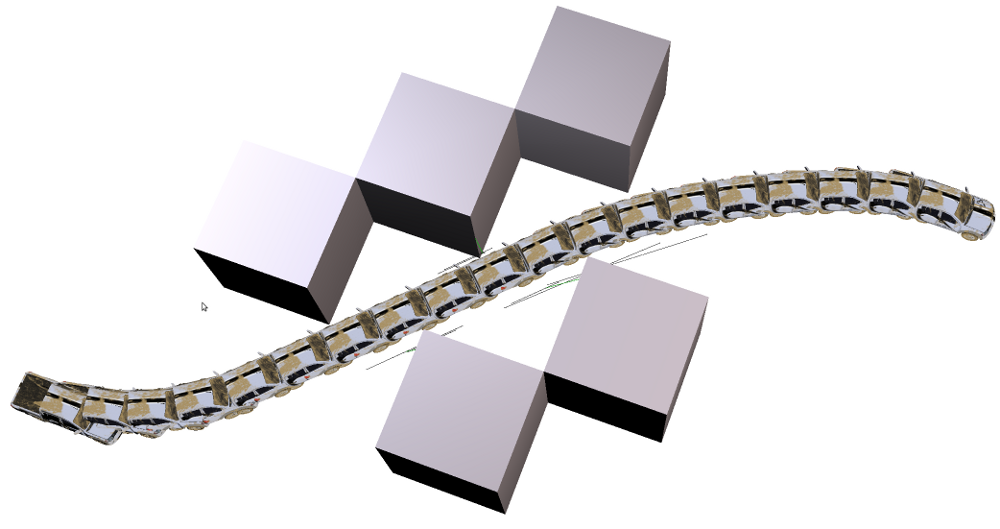
\includegraphics[width=0.26\linewidth]{figure/benchmark/jagged_dubins.png}} \qquad
\subfloat[gap-dubin]{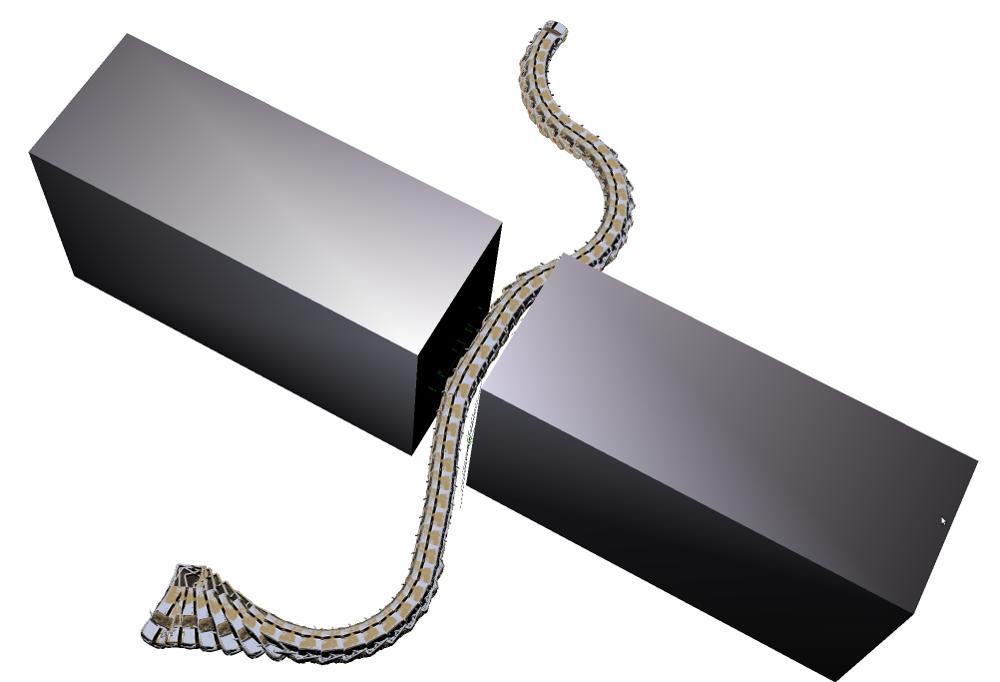
\includegraphics[width=0.21\linewidth]{figure/benchmark/cargap_dubins.png}} \qquad
\subfloat[squared-dubin]{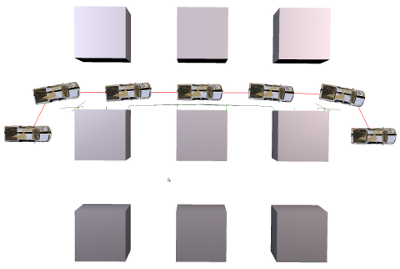
\includegraphics[width=0.22\linewidth]{figure/benchmark/squared_dubins.png}}
\caption{The dubins car environment for 2D experiments}
\label{fig:benchmarks1}
\end{figure*}

\begin{figure*}[t]
\centering
\subfloat[bookshelf]{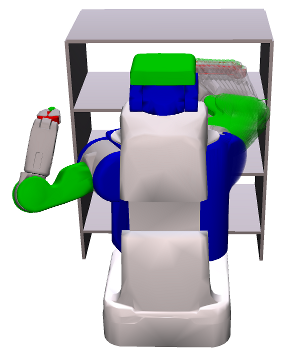
\includegraphics[width=0.12\linewidth]{figure/benchmark/bookshelves.png}} \qquad
\subfloat[skew-bookshelf]{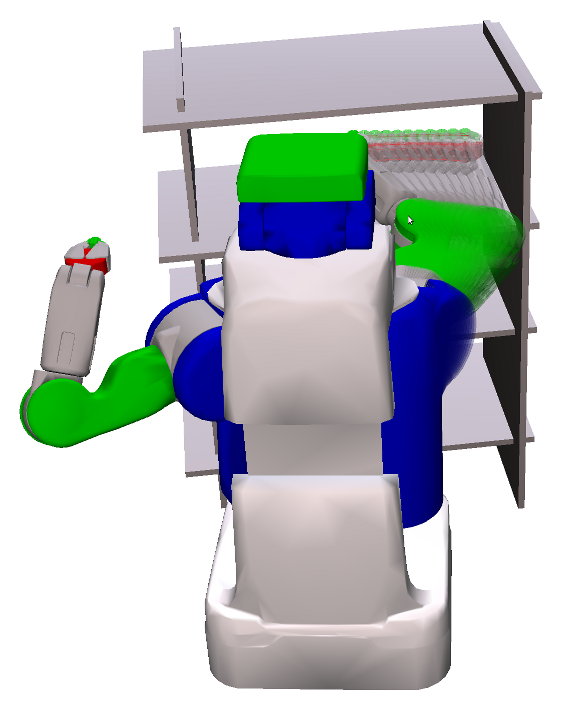
\includegraphics[width=0.12\linewidth]{figure/benchmark/bookshelves_rotate.png}} \qquad
\subfloat[countertop]{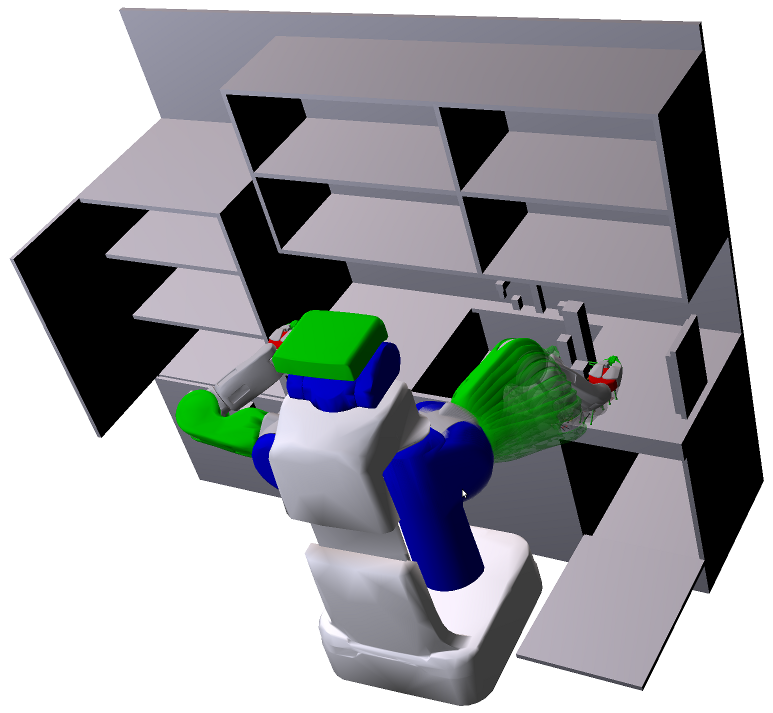
\includegraphics[width=0.16\linewidth]{figure/benchmark/countertop.png}} \qquad
\subfloat[industrial]{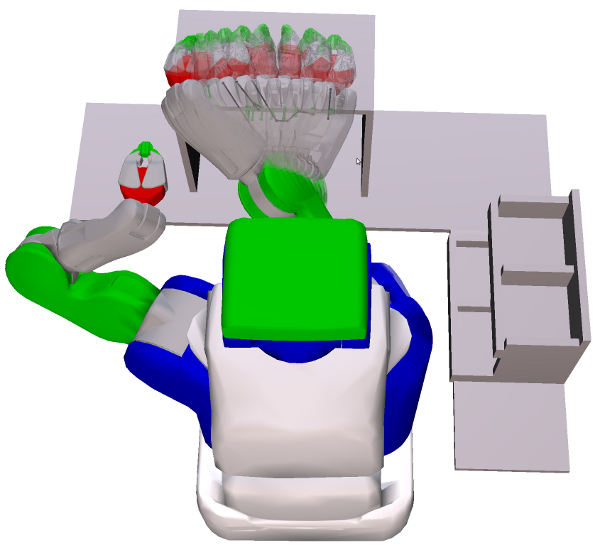
\includegraphics[width=0.16\linewidth]{figure/benchmark/industrial.png}} \qquad
\subfloat[industrial2]{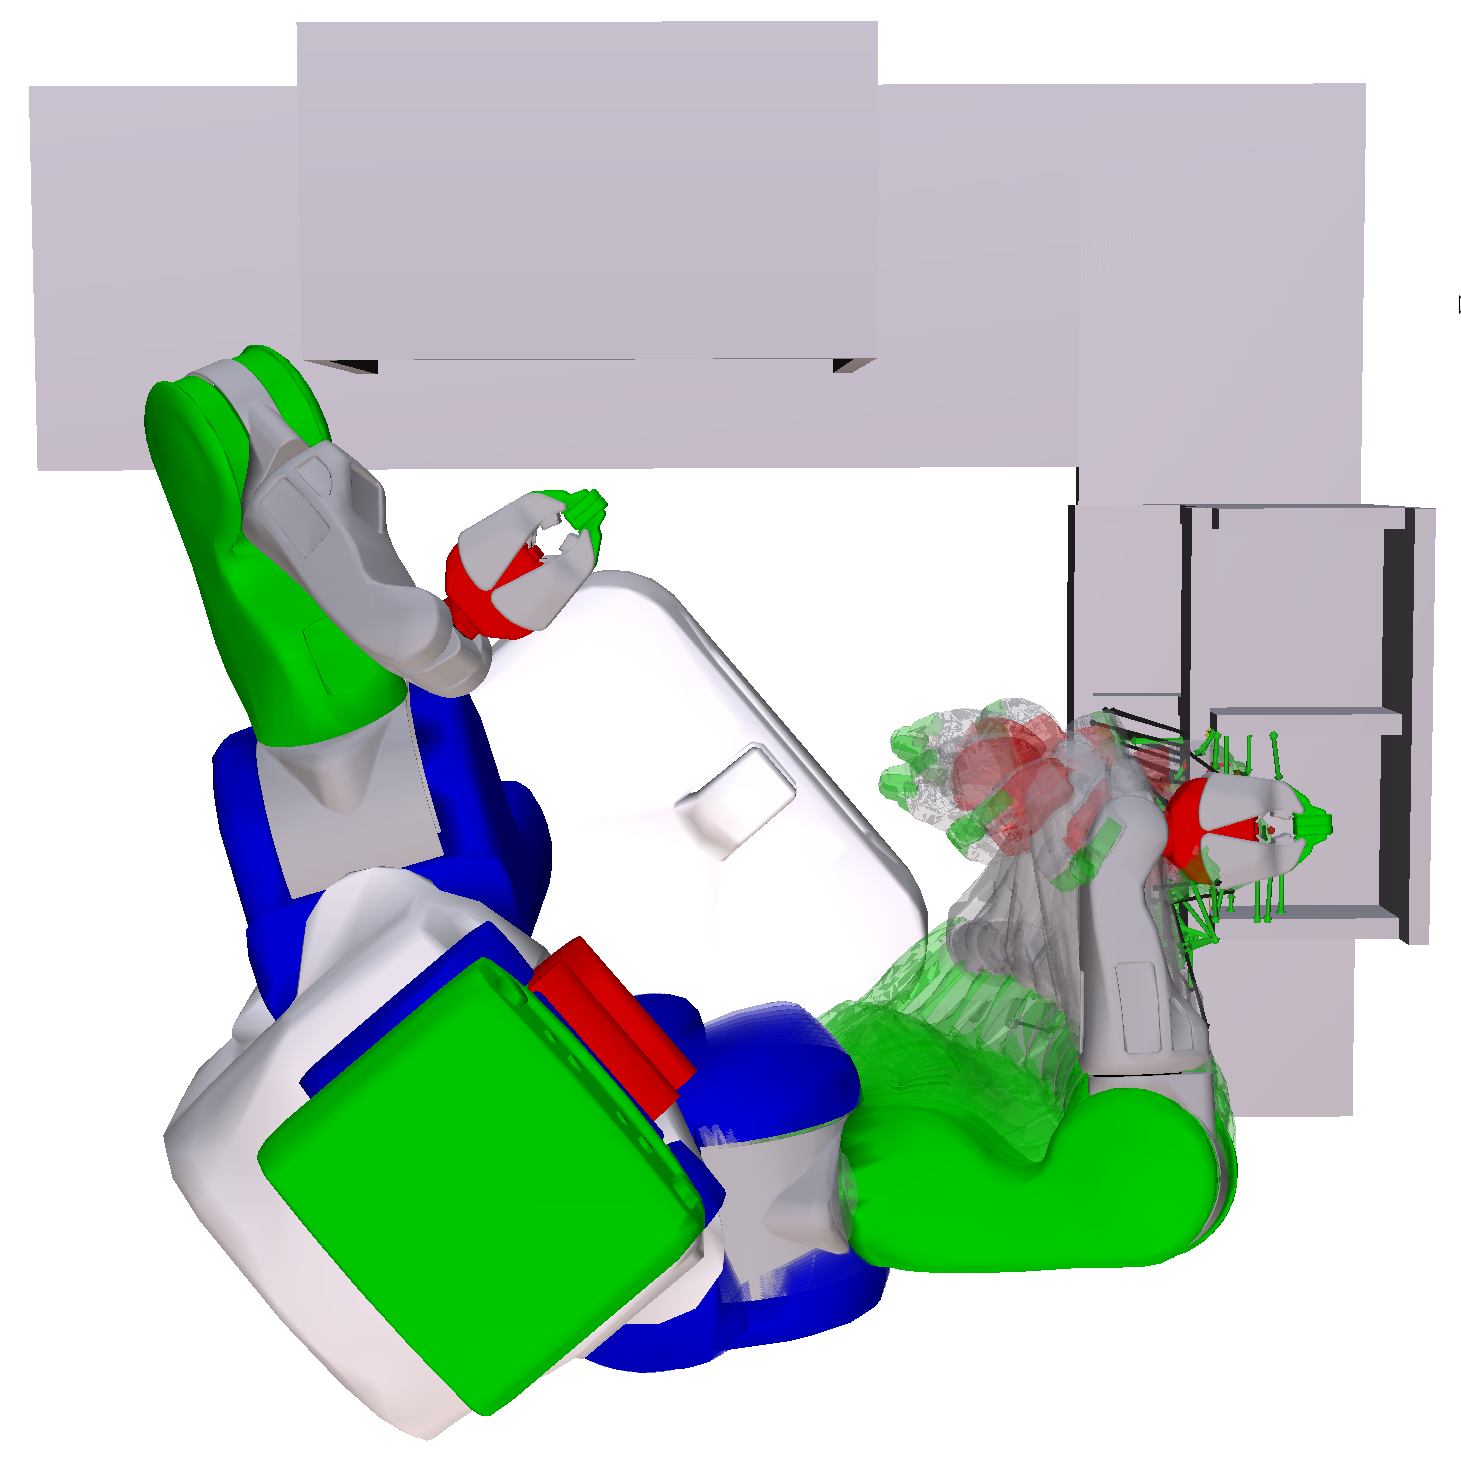
\includegraphics[width=0.14\linewidth]{figure/benchmark/industrial2.png}}
\caption{The PR2 benchmarks for right arm planning with 22 links.}
\label{fig:benchmarks2}
\end{figure*}


\begin{figure*}[t]
\centering
\subfloat[hotel]{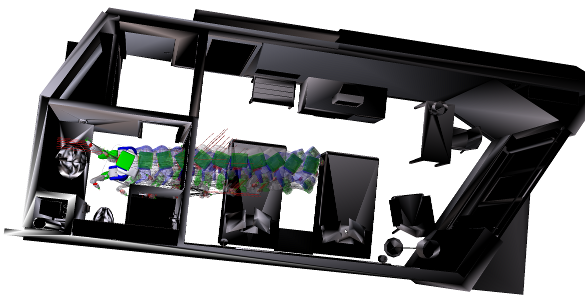
\includegraphics[width=0.28\linewidth]{figure/benchmark/hotel.png}} \qquad
\subfloat[kitchen]{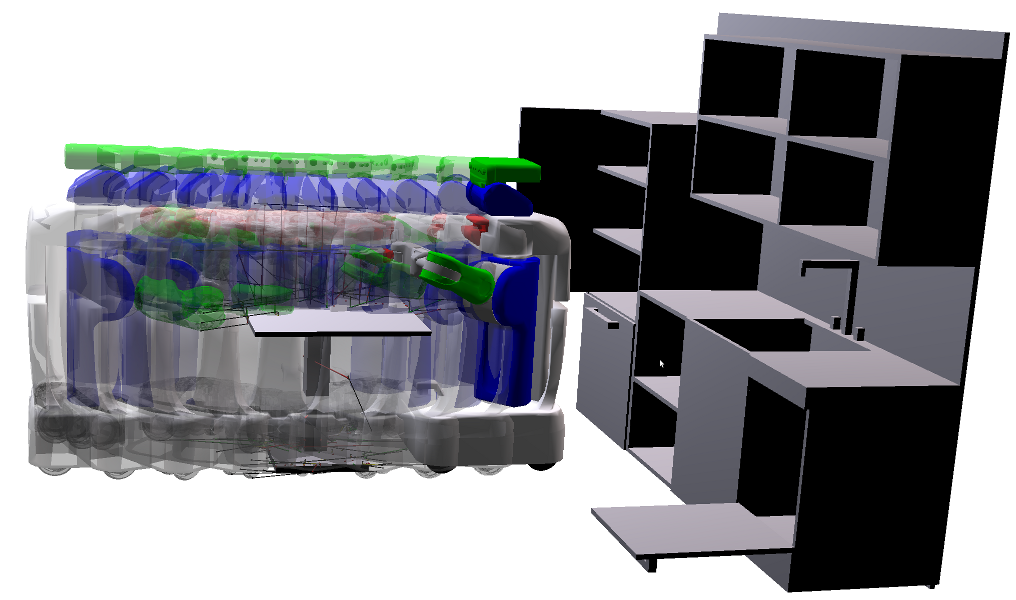
\includegraphics[width=0.26\linewidth]{figure/benchmark/kitchen10.png}} \\
\subfloat[kitchen2]{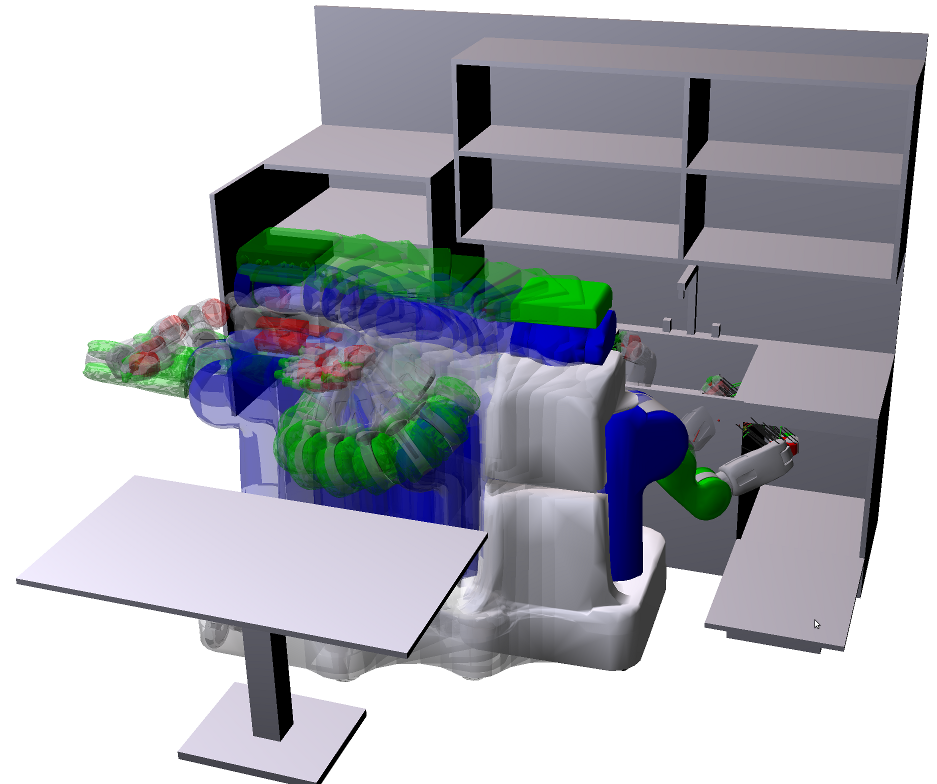
\includegraphics[width=0.19\linewidth]{figure/benchmark/kitchen.png}} \qquad
\subfloat[livingroom]{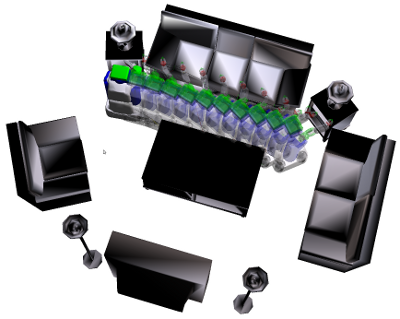
\includegraphics[width=0.19\linewidth]{figure/benchmark/livingroom.png}} \qquad
\subfloat[livingroom2]{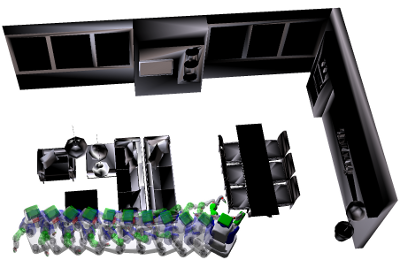
\includegraphics[width=0.24\linewidth]{figure/benchmark/livingroom2.png}}
\caption{The PR2 benchmarks for full-body planning with 88 links.}
\label{fig:benchmarks3}
\end{figure*}




\section{Conclusion}
In this paper, we have introduced novel features for trajectory effectiveness and demonstrated the trajectory effectiveness prediction algorithm based on these features. We showed the accuracy of the prediction algorithm on different planning tasks in various benchmarks. Additionally, we showed initial results on transferring the learned classifier to other benchmarks.

This work serves as a baseline of initial trajectory selection for trajectory optimization based motion planning. In future work, we would like to consider more combinations of trajectory features and explore more criteria for trajectory evaluation, including running time, objective value and cost for violated constraints. Moreover, instead of the qualitative metric used in this paper, we will apply regression algorithms to compute a quantitative evaluation for trajectory's effectiveness, which can be used for trajectory ranking during the optimization.
Finally, we will integrate the prediction algorithm with trajectory optimization, to improve both the performance and quality of the planning algorithm.


\section*{Acknowledgments}
This research has been funded in part by Darpa Young Faculty Award \#D13AP00046, and by a Sloan Fellowship.


\bibliographystyle{IEEEtran}
\bibliography{icra}

\end{document}
